%\documentclass[5p, times]{elsarticle}
\documentclass[review,number,sort&compress]{elsarticle}

%%%%%%%%%%%%%%   Preample  %%%%%%%%%%%%%%%%%%
%% for comment (texts in between \begin{comment} and \end{comment} will be ignored)
\usepackage{comment} 

%% The amssymb package provides various useful mathematical symbols
\usepackage{amssymb}
%% The amsthm package provides extended theorem environments
\usepackage{amsthm}

%% for celcius symbol
\usepackage{textcomp}

%% for units
\usepackage{siunitx}

%% multirow
\usepackage{multirow}

%% The lineno packages adds line numbers. Start line numbering with
%% \begin{linenumbers},  end it with \end{linenumbers}. Or switch it on
%% for the whole article with \linenumbers.
\usepackage{lineno}
\linenumbers

%% package for subfigure environment
\usepackage{subcaption}

%% package for type Greek letters without entering into math-mode
\usepackage{textgreek}

%% package for large picture in two-colume
\usepackage{dblfloatfix}
\usepackage{fixltx2e}
\usepackage{float}
%\usepackage{placeins}
\usepackage{subcaption}

%% only jpg pdf eps are allowed, tiff format are not allowed in latex
%% eps in principle can't be compiled by pdflatex, pdf not compiled by latex, but Kile can do some intermedate conversion to allow this happen.
\DeclareGraphicsExtensions{.pdf, .eps, .jpg}
%%opening
\journal{NIMA}

\begin{document}

%%%%%%%%%%%%%% Front Matter %%%%%%%%%%%%%%%%%%
\begin{frontmatter}

\title{A versatile PMT test bench and its application in the PSD detector of DAMPE}
%%\title{Title with footnote\tnoteref{t1}}
%%\tnotetext[t1]{FootNote for title}

\author[imp,lzu,ucas]{Yong Zhou}
%\ead{yong@impcas.ac.cn}

\author[imp]{Yuhong Yu}
%%\ead{yuyuhong@impcas.ac.cn}

\author[imp]{Zhiyu Sun\corref{corresponding_author}}
\cortext[corresponding_author]{Corresponding author}
\ead{sunzhy@impcas.ac.cn}

\author[lzu]{Bitao Hu}
%% Additional Author information %%
%%\author[ano]{Anonymous\fnref{fn1}}
%%\ead{anonymous@anonymous.cn}
%%\fntext[fn1]{FootNote for Anonymous author}

\address[imp]{Institute of Modern Physicas, Chinese Academy of Sciences,  509 Nanchang Road,  Lanzhou,  730000,  P.R.China}
\address[lzu]{School of Nuclear Science and Technology,  Lanzhou University,  222 South Tianshui Road,  Lanzhou,  730000,  P.R.China}
\address[ucas]{Graduate University of the Chinese Academy of Sciences,  19A Yuquan Road,  Beijing,  100049,  P.R.China}
%%\address[ano]{Anonymous Address of Anonymous author}

%%
\begin{abstract}

A versatile test bench, dedicated for massive PMT characterization, is developped at the Institute of Modern Physics, Chinese Academy of Sciences.
The test bench is suitable for reuse in different applications and incorporates the cathode surface scanning as its intrinsic capability.
Initial application of the test bench in the Plastic Scintillator Strip Detector of DArk Matter Paricle Explorer is successfull and a total of 570 Hamamastu R4443 Mod2 tubes have been charaterized.
Implementation details of the test bench is described in this article.
Major results and performance of the test bench during this application are also reported. 
\end{abstract}

%%
\begin{keyword}
Photomultiplier
\sep PMT
\sep PSD
\sep DAMPE

%% PACS codes here,  in the form: \PACS code \sep codes

%% MSC codes here,  in the form: \MSC code \sep code
%% or \MSC[2008] code \sep code (2000 is the default)

\end{keyword}

\end{frontmatter}

%%%%%%%%%%%%%%%%  Introduction  %%%%%%%%%%%%%%%%%%%%%%%
\section{Introduction}
\label{sec:introduction}

%%Photomultiplier tubes(PMTs) are widely used as photosensors in various fields, such as particle detectors in experimental physics and medical equipments in medical diagnosis.
%%PMT features in high sensitivity, large gain and easy-operation, whic make it still popular about 80 years after its invention.
Photomultiplier tubes(PMTs) are widely used as photosensors in particle detectors.
Modern detectors can easily contain hundreds, even thousands of PMTs as detection channels.
PMTs ususally need to be charaterized thoroughly in the laboratoy before use, as the parameters provided by the manufacturer only give a rough indication of the performance.
These tests are critical for the following reasons:
\begin{itemize}
 \item Each experiment has its specific requirements for the characteristics of PMT.
 As PMTs exhibit large individual difference, these parameters should be measured and selection based on the measurement result should be performed to reject tubes that are out of the specification.
 \item To obtain a uniform response across the whole detector and thus optimize the performance, the response of PMT as a function of supplying voltage, sometimes of the cathode position, need to be determined.
  These data is invaluable for both the construction and operation of the detector. 
 \item Last but not least, qualification test of the whole PMT assembly before final mounting is mandatory for the success of any large experiment. 
\end{itemize}

Massive testing of large number of PMTs is a tough job.
Usually, a dedicated test bench is constructed to facilitate this work~\cite{barnhill_testing_2008,akgun_complete_2005,adragna_pmt-block_2006}.
Setting up a system like this is none trivial work, which demands considerable investment of time and effort.
On the other hand, testing of PMTs is a commonly encountered procedure and many components of the testing configuration can be shared among different applications.
%Thus, it is desirable that the same test bench, with minimum configuration changes, can be reused in different applications. 

In this paper, a versatile test bench dedicated for PMT characterization is reported.
The test bench is designed to be a standard laboratoy equipment for fast PMT characterization for several experiments prepared and planned at the Institute of Modern Physics(IMP), Chinese Academy of Sciences.
To accommodate the various requirements of different experiments, the test bench has adoptted a modular design pattern both in the hardware and the associated software platform.
This makes the migration from one testing configuration to another light-weight and time-saving.
Design considerations of the test bench and detailed description of its implementation are presented in Sec.\ref{sec:design_consideration} and Sec.\ref{sec:description} respectively.

Initial application of the test bench in the PMT testing for the Plastic Scintillator Strip Detector(PSD) of DArk Matter Paricle Explorer(DAMPE)~\cite{Chang_Jin_dampe} is reported in Sec.\ref{sec:application}.
DAMPE is a statellite-borne  exeperiment, which imposes severe testing procedure for the PMT used.
PSD is a large-area two-layer plastic scintillator array which aims for  e/$\gamma$ discrimination as well as charge measurement up to Z=20 by measuring the energy deposited.
%%PSD requires a \SI{25}{\percent} energy uniformity across all the detection units.
%%Totally, 570 PMTs are charaterized and 194 of them are selected for production and qualification.
This application is successfull and has verified the efficiency and stability of the test bench.
Performance of the test bench has been extracted from these tests and is discussed in Sec.\ref{sec:summary}.

\section{Considerations in the design of the test bench}
\label{sec:design_consideration}
%\begin{comment}
\begin{figure*}
 \centering
 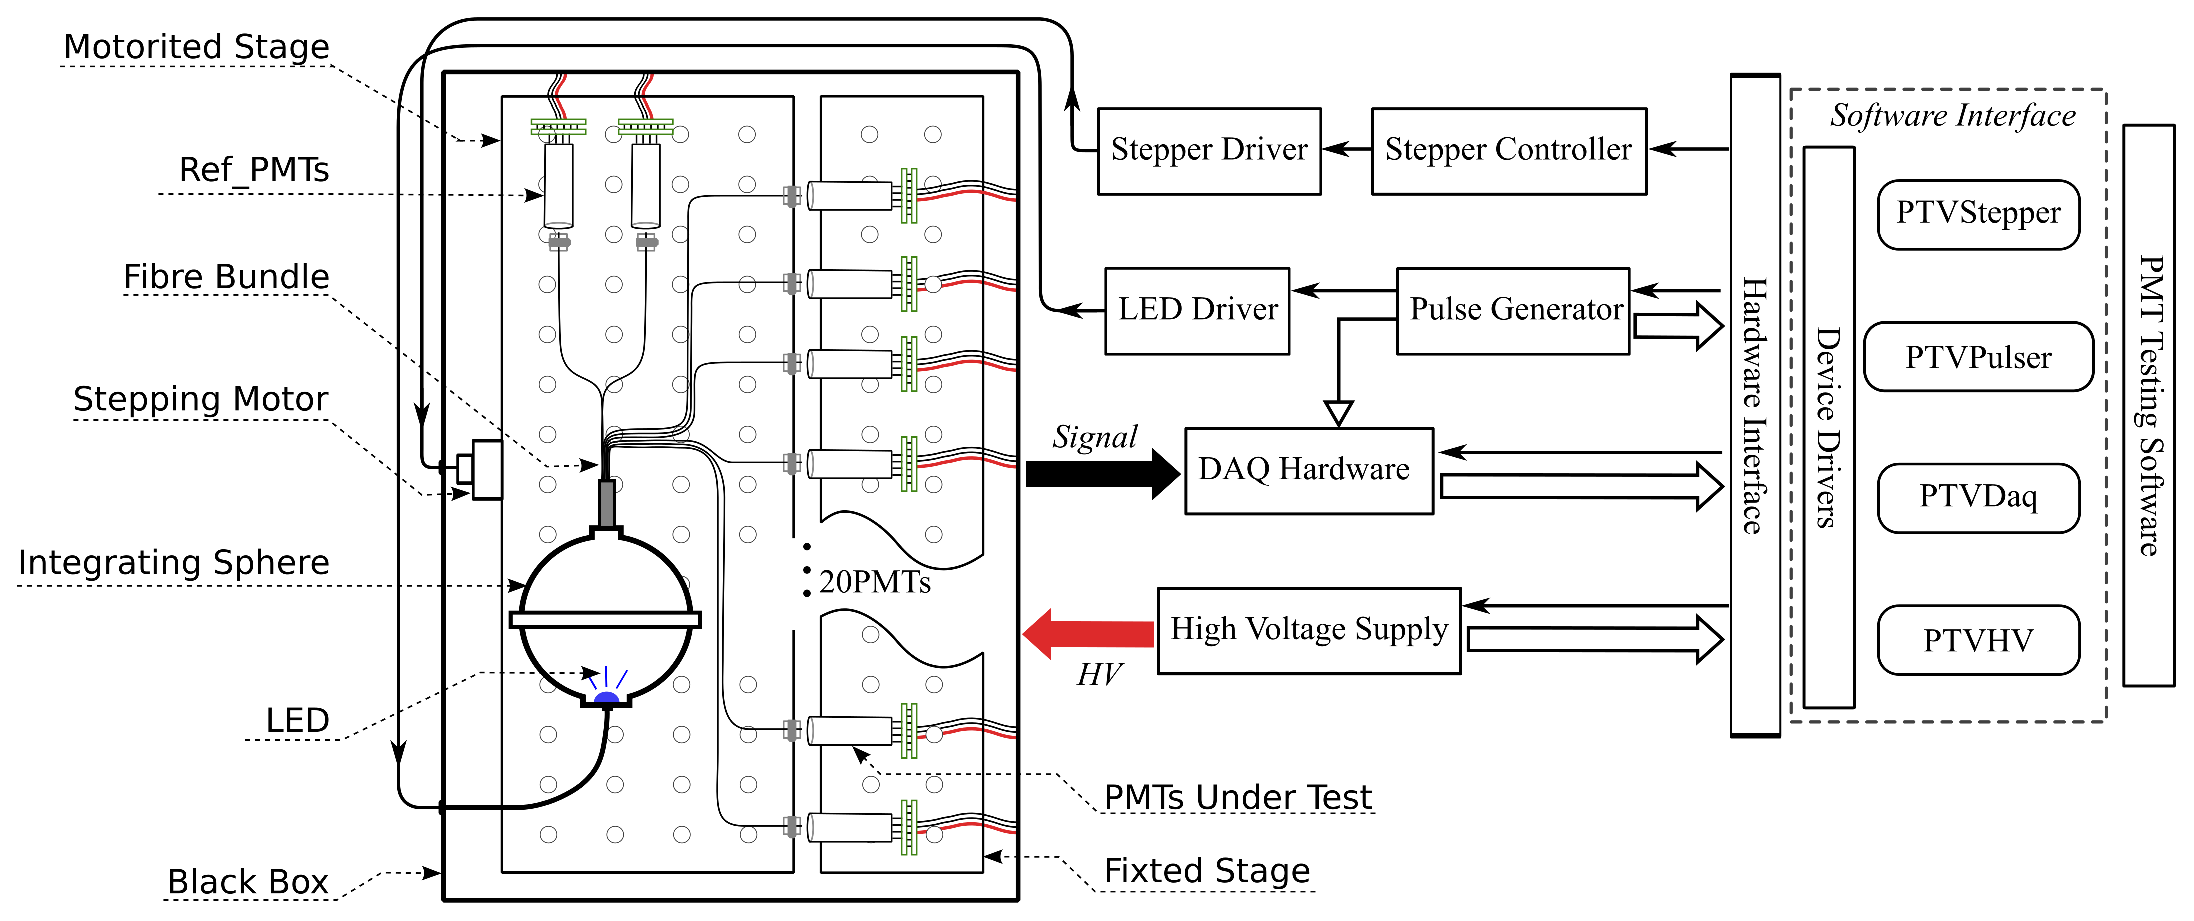
\includegraphics[width=160mm]{testbench_overview}
\caption{Schematic diagram of the PMT test bench system.}
\label{fig:testbench_overveiw}
\end{figure*}
%\end{comment}

The major design considerations of the test bench is summarized as follows:
\begin{itemize}
 \item \textit{Large capacity}: This is the primary driving force for developping a test bench dedicated for PMT characterization.
 Testing multiple tubes simultaneously can increase the efficiency and save project time tremendously.
 This is a critical factor in large experiments involving large number of PMTs.
 \item \textit{Automation}: A single test run for PMT characterization ususally takes several hours, during which most operations are trivial jobs like changing voltage, changing light intensity and so on.
 Manual operations are inefficient and unreliable in such a long period.
 Computer controllable hardwares should be used whenever possible and corresponding software should be developped to automate these trivial operations.
 Manual intervention is only expected in the beginning when mounting PMTs and configuring the software and in the end when unmounting PMTs and assessing testing result. 
 \item \textit{Versatility}: The test bench is not designed for single use.
 %It will be utilitized in different experiments with different testing requirements.
 T\-h\-u\-s potential use cases should be considered and appropriate hardwares should be set up in the first place.
 In particular, cathode surface scanning capability is desirable in use cases like TOF-PET~\cite{tof_pet} where multiple scintillators are coupled to a single position-sensitive PMT(PSPMT) or multi-anode PMT(MAPMT). 
 \item \textit{Flexibility}: As a by product of versatiltiy, flexibility is needed both in terms of hardware and software.
 The hardware platform should be extensible and allow complex testing configurations.
 The software should accommodate any changes in the hardware easily, while keeping the high level functionality unchanged and portable. 
\end{itemize}


%%%%%%%%%%%%%%%% Main Text Body %%%%%%%%%%%%%%%%%%%%%%%
\section{Description of the test bench}
\label{sec:description}

A schematic diagram of the final design is shown in Fig.\ref{fig:testbench_overveiw}.
The test bench can test up to 25 PMTs in a single run.
Light pulses are distributed to each tube through an integrating sphere and a fibre bundle, which are mounted on a three-dimensional motorized stage.
PMTs under test will be mounted on a separate fixed stage, thus allowing position scanning of all tubes simultaneously.
Two additional PMTs are mounted on the motorized stage, serving as reference to monitor the stability of the light source as well as the performance of the whole system(see Sec.\ref{sec:summary}).
They will move with the light distribution system and not be removed from their fixed positions during all test runs. 
Both stages are housed in a light-tight box made of aluminium alloy, with the dimension of $176cm\times100cm\times78cm$.
The box is painted black inside and out and can be opened from the top plate for tube mounting.
Cables are led out through light-tight cable feedthroughs left in the side plate.

Controlling devices of the test bench are located outside the light-tight box.
They are grouped into four types according to the functions, i.e. motion controller, pulse generator, data acquisition system(DAQ) and high voltage supply.
Pulse generator is used to generate trigger pulses to the LED driver as well as to the DAQ electronics simultaneously.
%Four types of devices, i.e. motion controller, pulse generator, data acquisition system(DAQ) and high voltage supply, are recognized as the essential parts of the test bench system.
%In particular, pulse generator not only 
These four types of devices are needed in every basic PMT characterization and are considered as the essential parts of the test bench system.
%They are needed in every basic PMT characterization, however different hardware may be used in different applications.
Motion controller and pulse generator can be shared among different applications as they are tightly coupled to the test bench itself.
On the other hand, DAQ and high voltage supply have direct relation to the PMTs under test and are expected to undergo frequent replacement.
It's a common practise that project-specific hardware be used for PMT characterization in large experiments, as in the case of DAMPE PSD(see Sec.\ref{sec:application}).
%While motion controller and pulse generator can be shared, different hardware for the DAQ and high voltage supply may be utilized in different applications.
For laboratoy routine test, a universal CAMAC system based on CC-USB crate controller~\cite{cc_usb} and a CAEN SY1527LC power crate~\cite{sy1527lc} have been set up and ready to use.

All devices are controlled by a single software.
Changing of hardware is handled smoothly in the software design and automation is realized in every aspect of the test bench.
%All other devices are located outside the light-tight box.

The whole test bench system is sitted in a cleanroom of ISO class 8 at IMP.
Temperature of the room is controlled around 22\textpm~2\textcelsius~all the time.
In the following, key components of the test bench will be described in detail.

%\begin{comment}
\begin{figure}
 \centering
 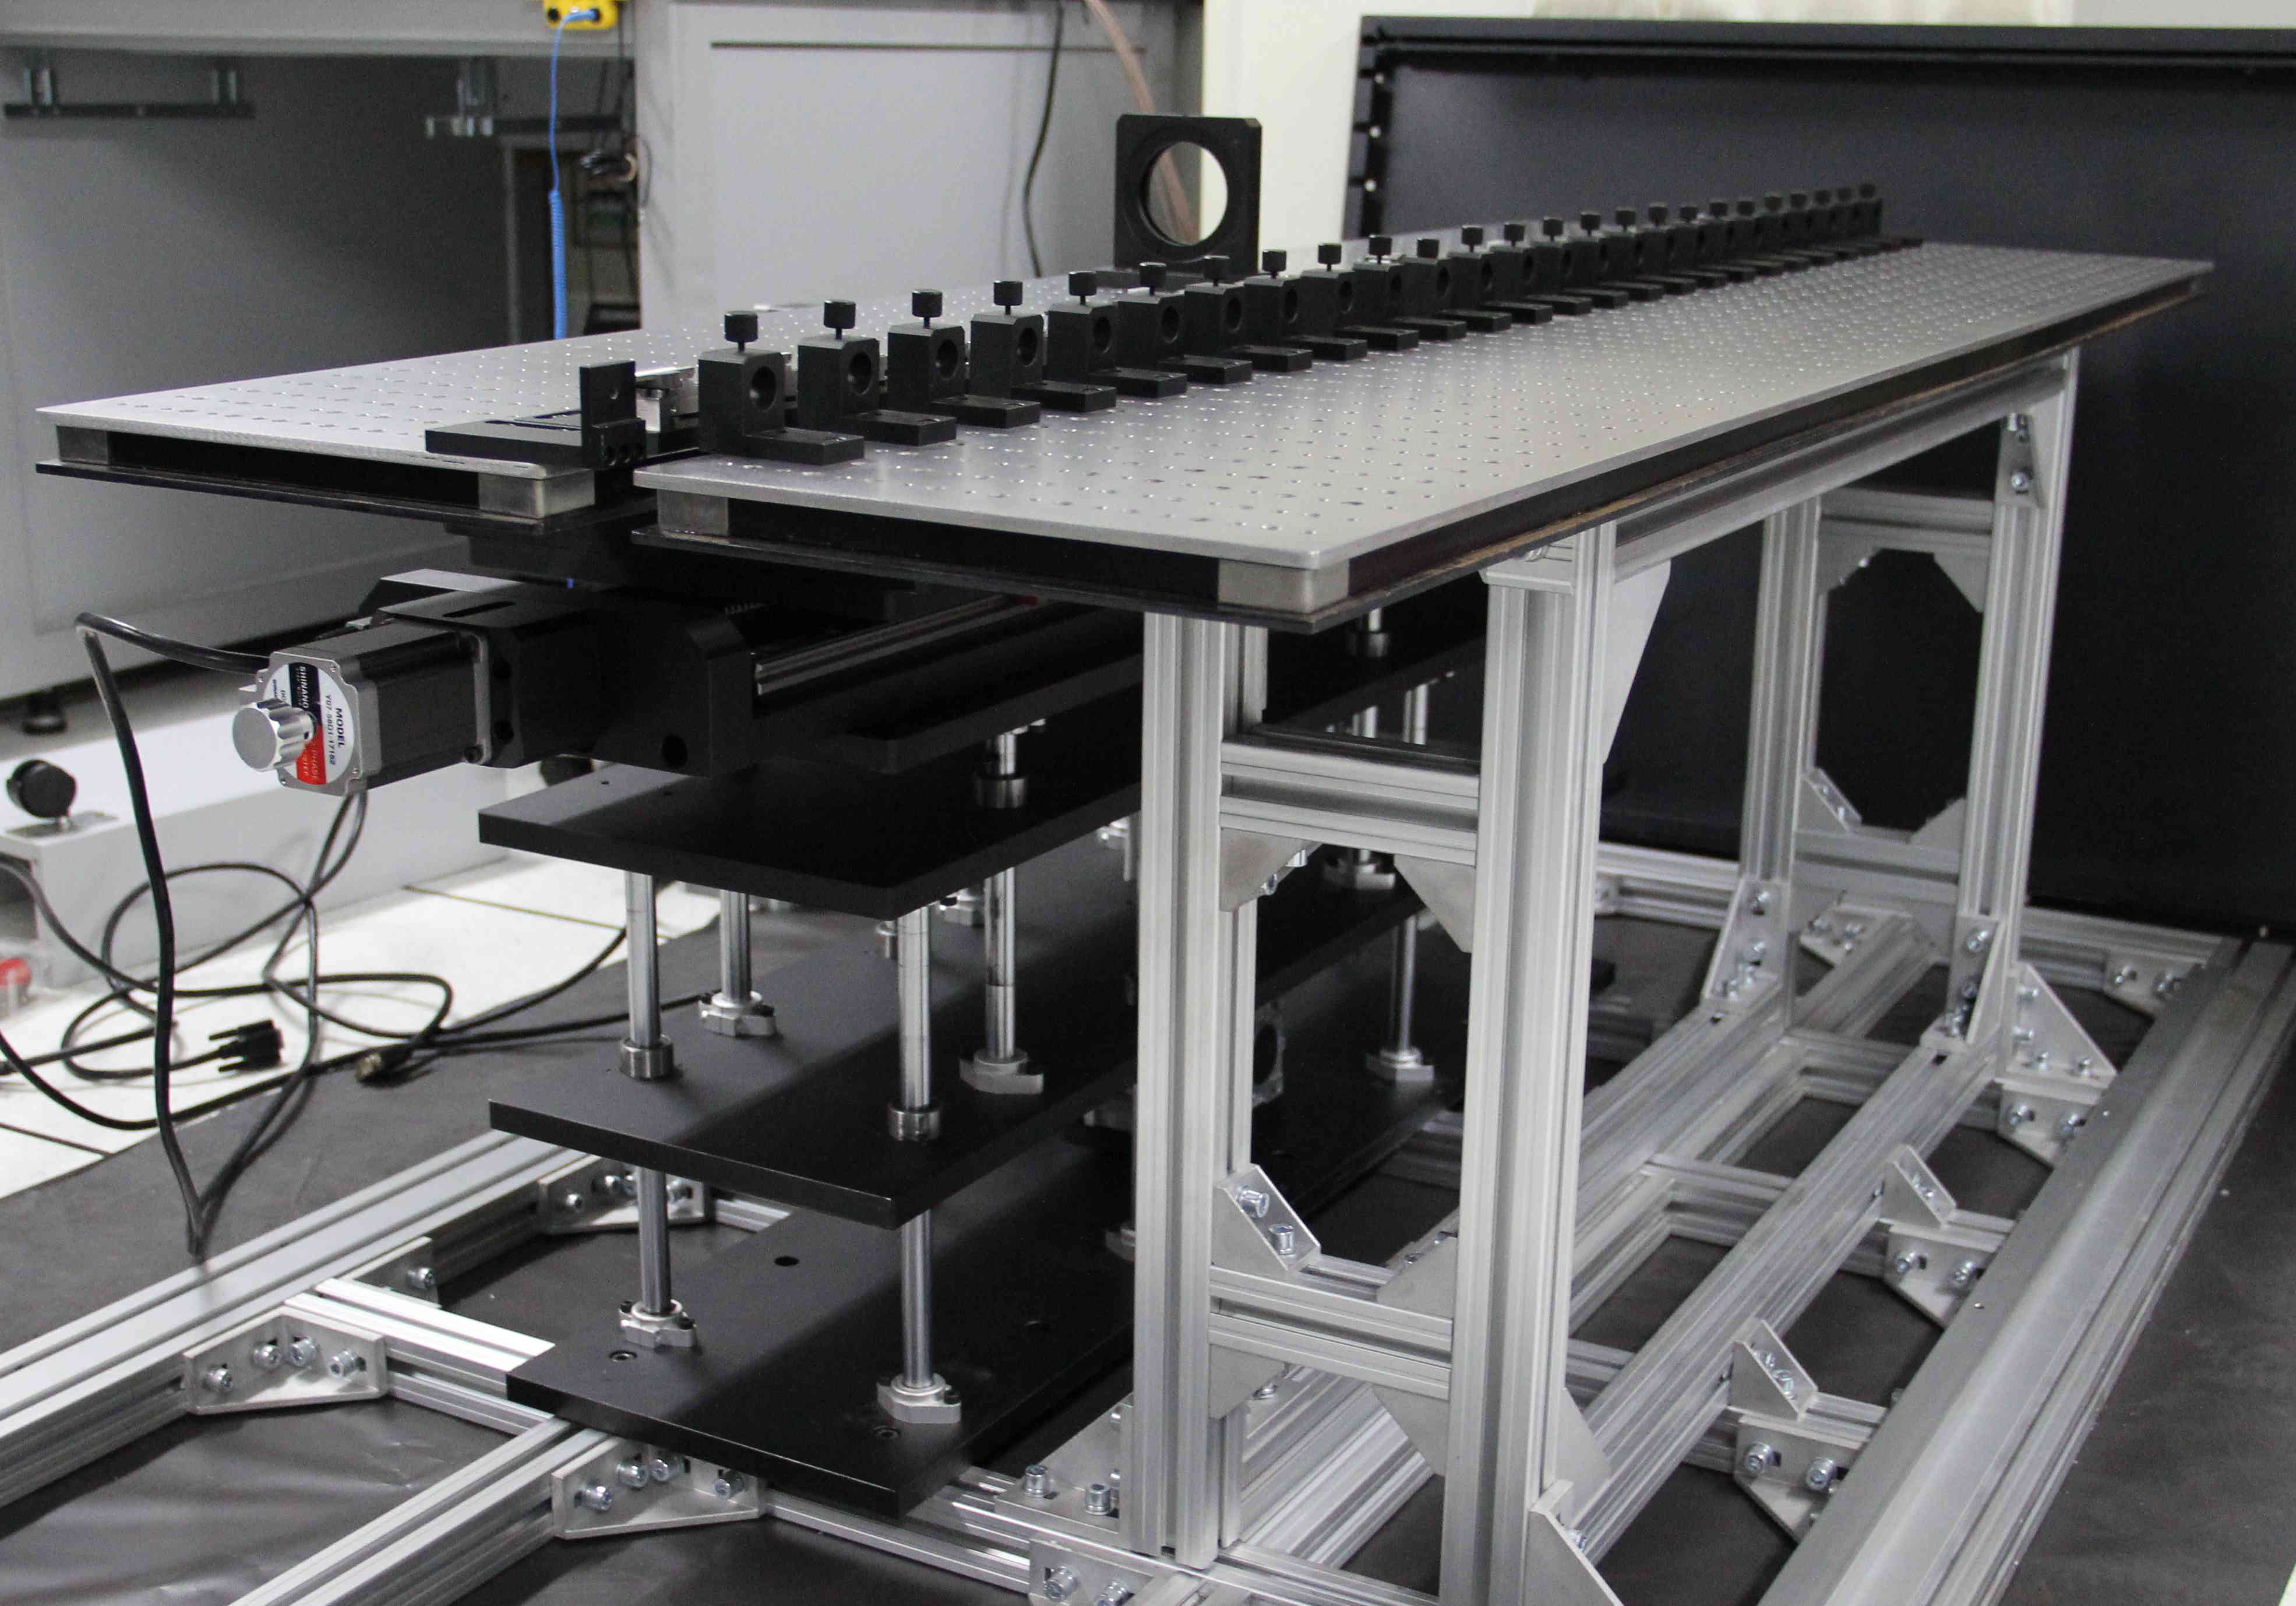
\includegraphics[width=90mm]{stage1_crop}
\caption{Motorized and fixed stages before assembly.
Fixtures for integrationg sphere, fibres and PMTs can be seen on top of them.}
\label{fig:stages}
\end{figure} 
%\end{comment}

\subsection{Motorized and Fixed Stages}
\label{sec:stages}

The motorized and fixed stages are the main body of the test bench.
All other objects inside the light-tight box will be mounted on the top of them.
In particular, customized fixtures for fibres, tubes and integration sphere have been designed for convenient and accurate poistioning.

The stages are arranged face to face with each other and both covered with an optical breadboard of an area $1560mm\times250mm$, as shown in Fig.\ref{fig:stages}.
These boards are made of \SI{2.5}{cm} thick stainless steel, providing substantial resistance to deformation in this application.
The grid pattern of tapped holes on the surface of them not only facilitates mounting/unmounting operations, but also provides extra flexibility in the testing configuration setup.

The load capacity of the motorized stage is \SI{30}{\kilo\gram} and it is driven by three stepping motors with a minimum step of \SI{1.56}{\micro\meter}.% which is sufficient for all use cases.
The travel range in the horizontal direction and vertical direction is \SI{60}{\milli\meter} and \SI{70}{\milli\meter} respectively.%covering a maximum scanning area of $60mm\times60mm$.
Thus the maximum scanning area is $60mm\times60mm$, which covers the size of the majority of PSPMTs and MAPMTs.
The third direction with a travel range of $15mm$ is added to control the gap between the fibre and the tube's cathode surface.
This may also be useful when extra space is needed to unmount tubes without disturbing the optical fibres. 
Stepping motors are controlled by three stepper drivers together with a motion controller MPC07SP from Leetro~\cite{leetro}.
MPC07SP possesses a PCI interface for remote control.

%\begin{comment}
\begin{figure}
 \centering
 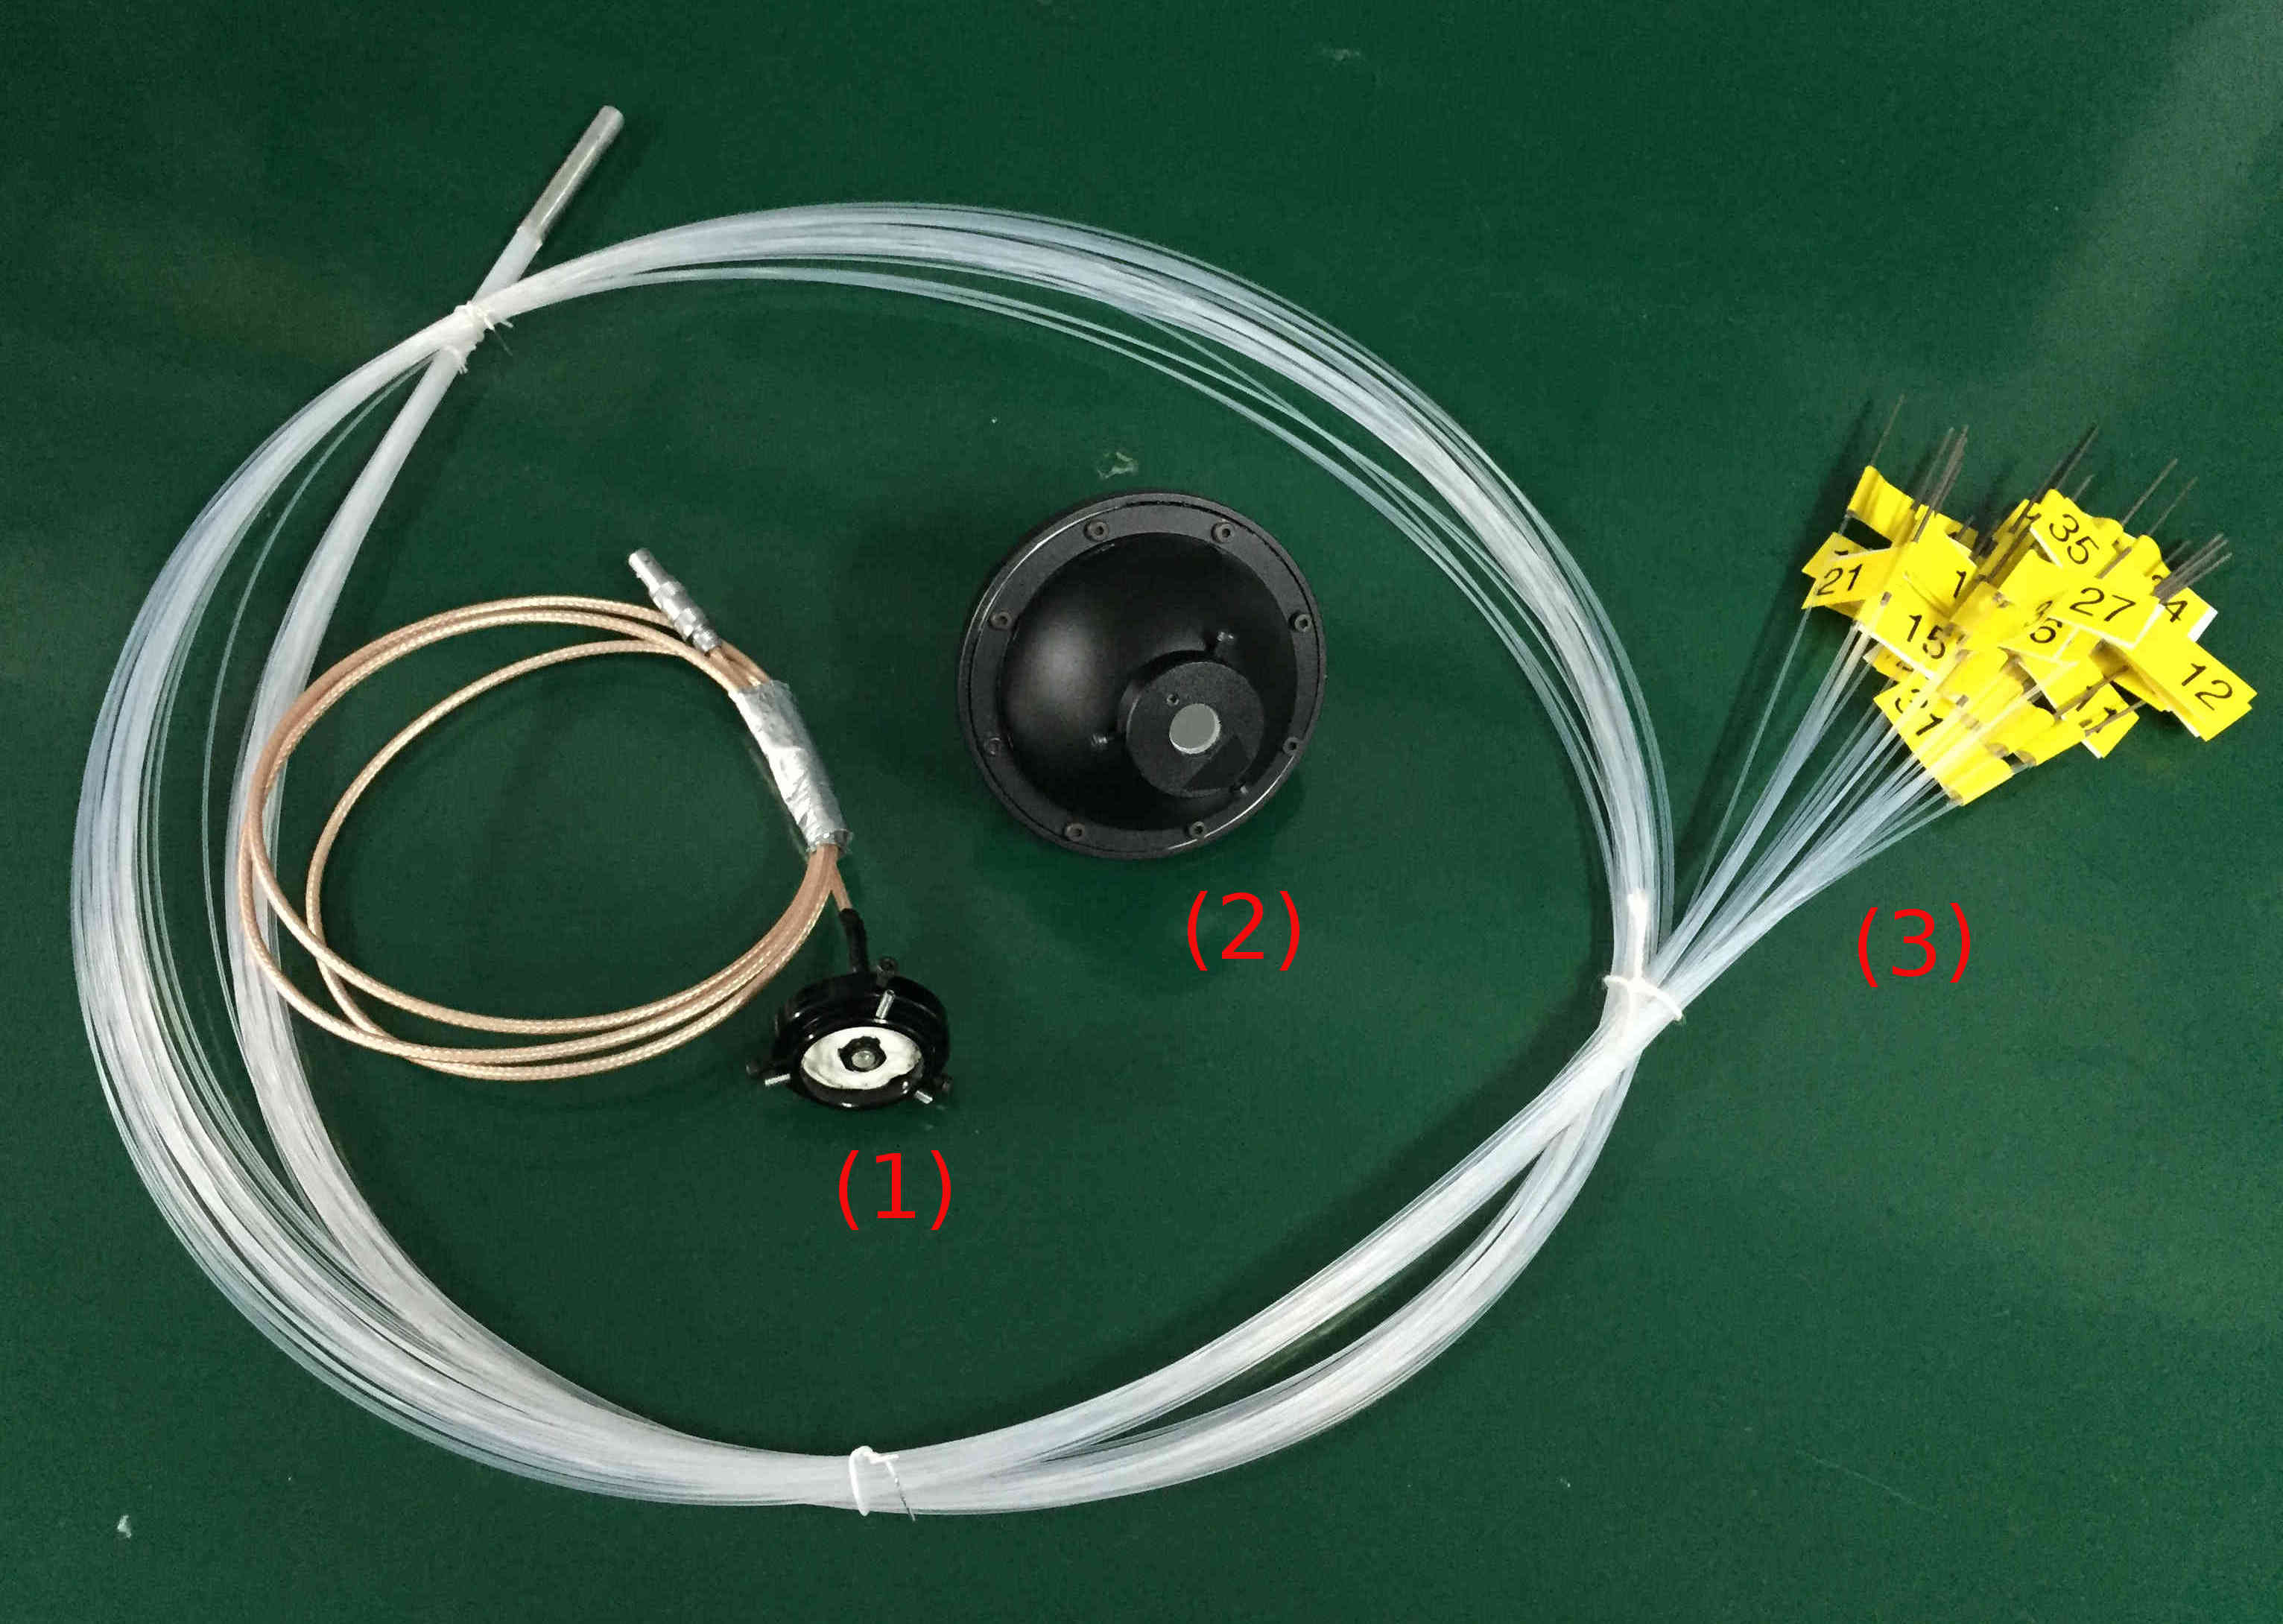
\includegraphics[width=90mm]{fibre_led_insphere_crop}
\caption{Components of the light distribution system:(1)LED glued to the base (2)Integrating sphere (3)Fibre bundle, labeled for each fibre}
\label{fig:fibre_led_sphere}
\end{figure} 

%\begin{comment}
\begin{figure}
 \centering
 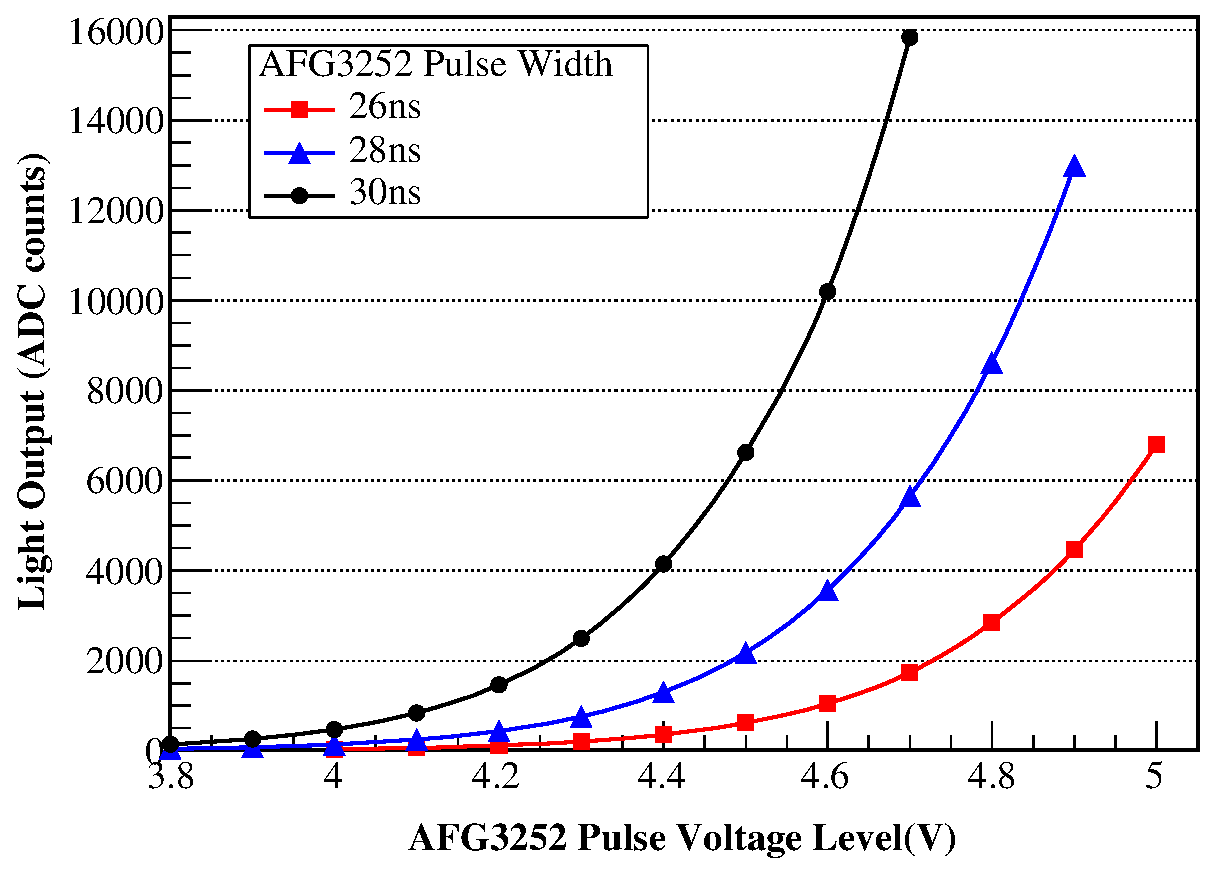
\includegraphics[width=90mm]{intesityVSvoltage}
\caption{Light intensity as a function of AFG3252 pulse voltage}
\label{fig:afg3252_intensityVSvoltage}
\end{figure} 
%\end{comment}

\begin{figure}
 \centering
 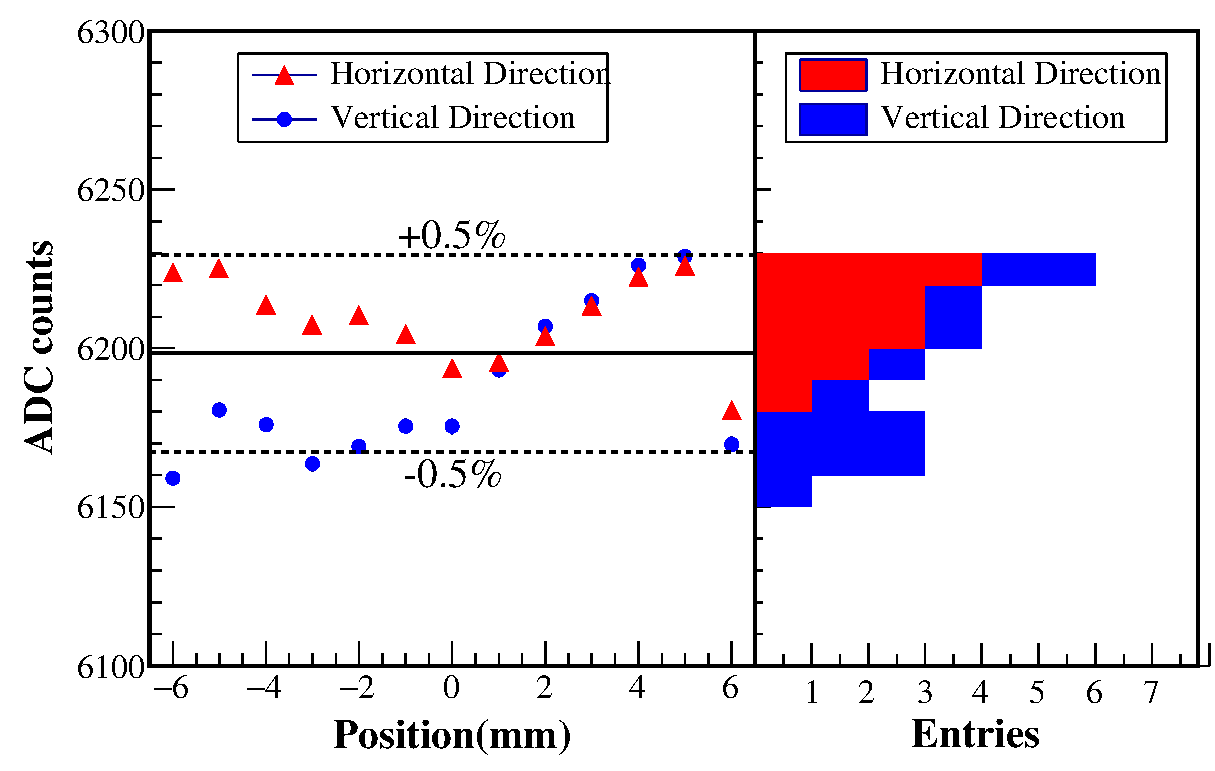
\includegraphics[width=90mm]{uniformity_integratingsphere}
\caption{Spatial uniformity of the integrating sphere.
The output port has a diameter of \SI{14}{\milli\meter}.
Central \SI{12}{\milli\meter} is scanned both in the horizontal and verical direction with a step of \SI{1}{\milli\meter}}
\label{fig:uniformity_integratingsphere}
\end{figure} 
%\end{comment}



\begin{figure}
 \centering
 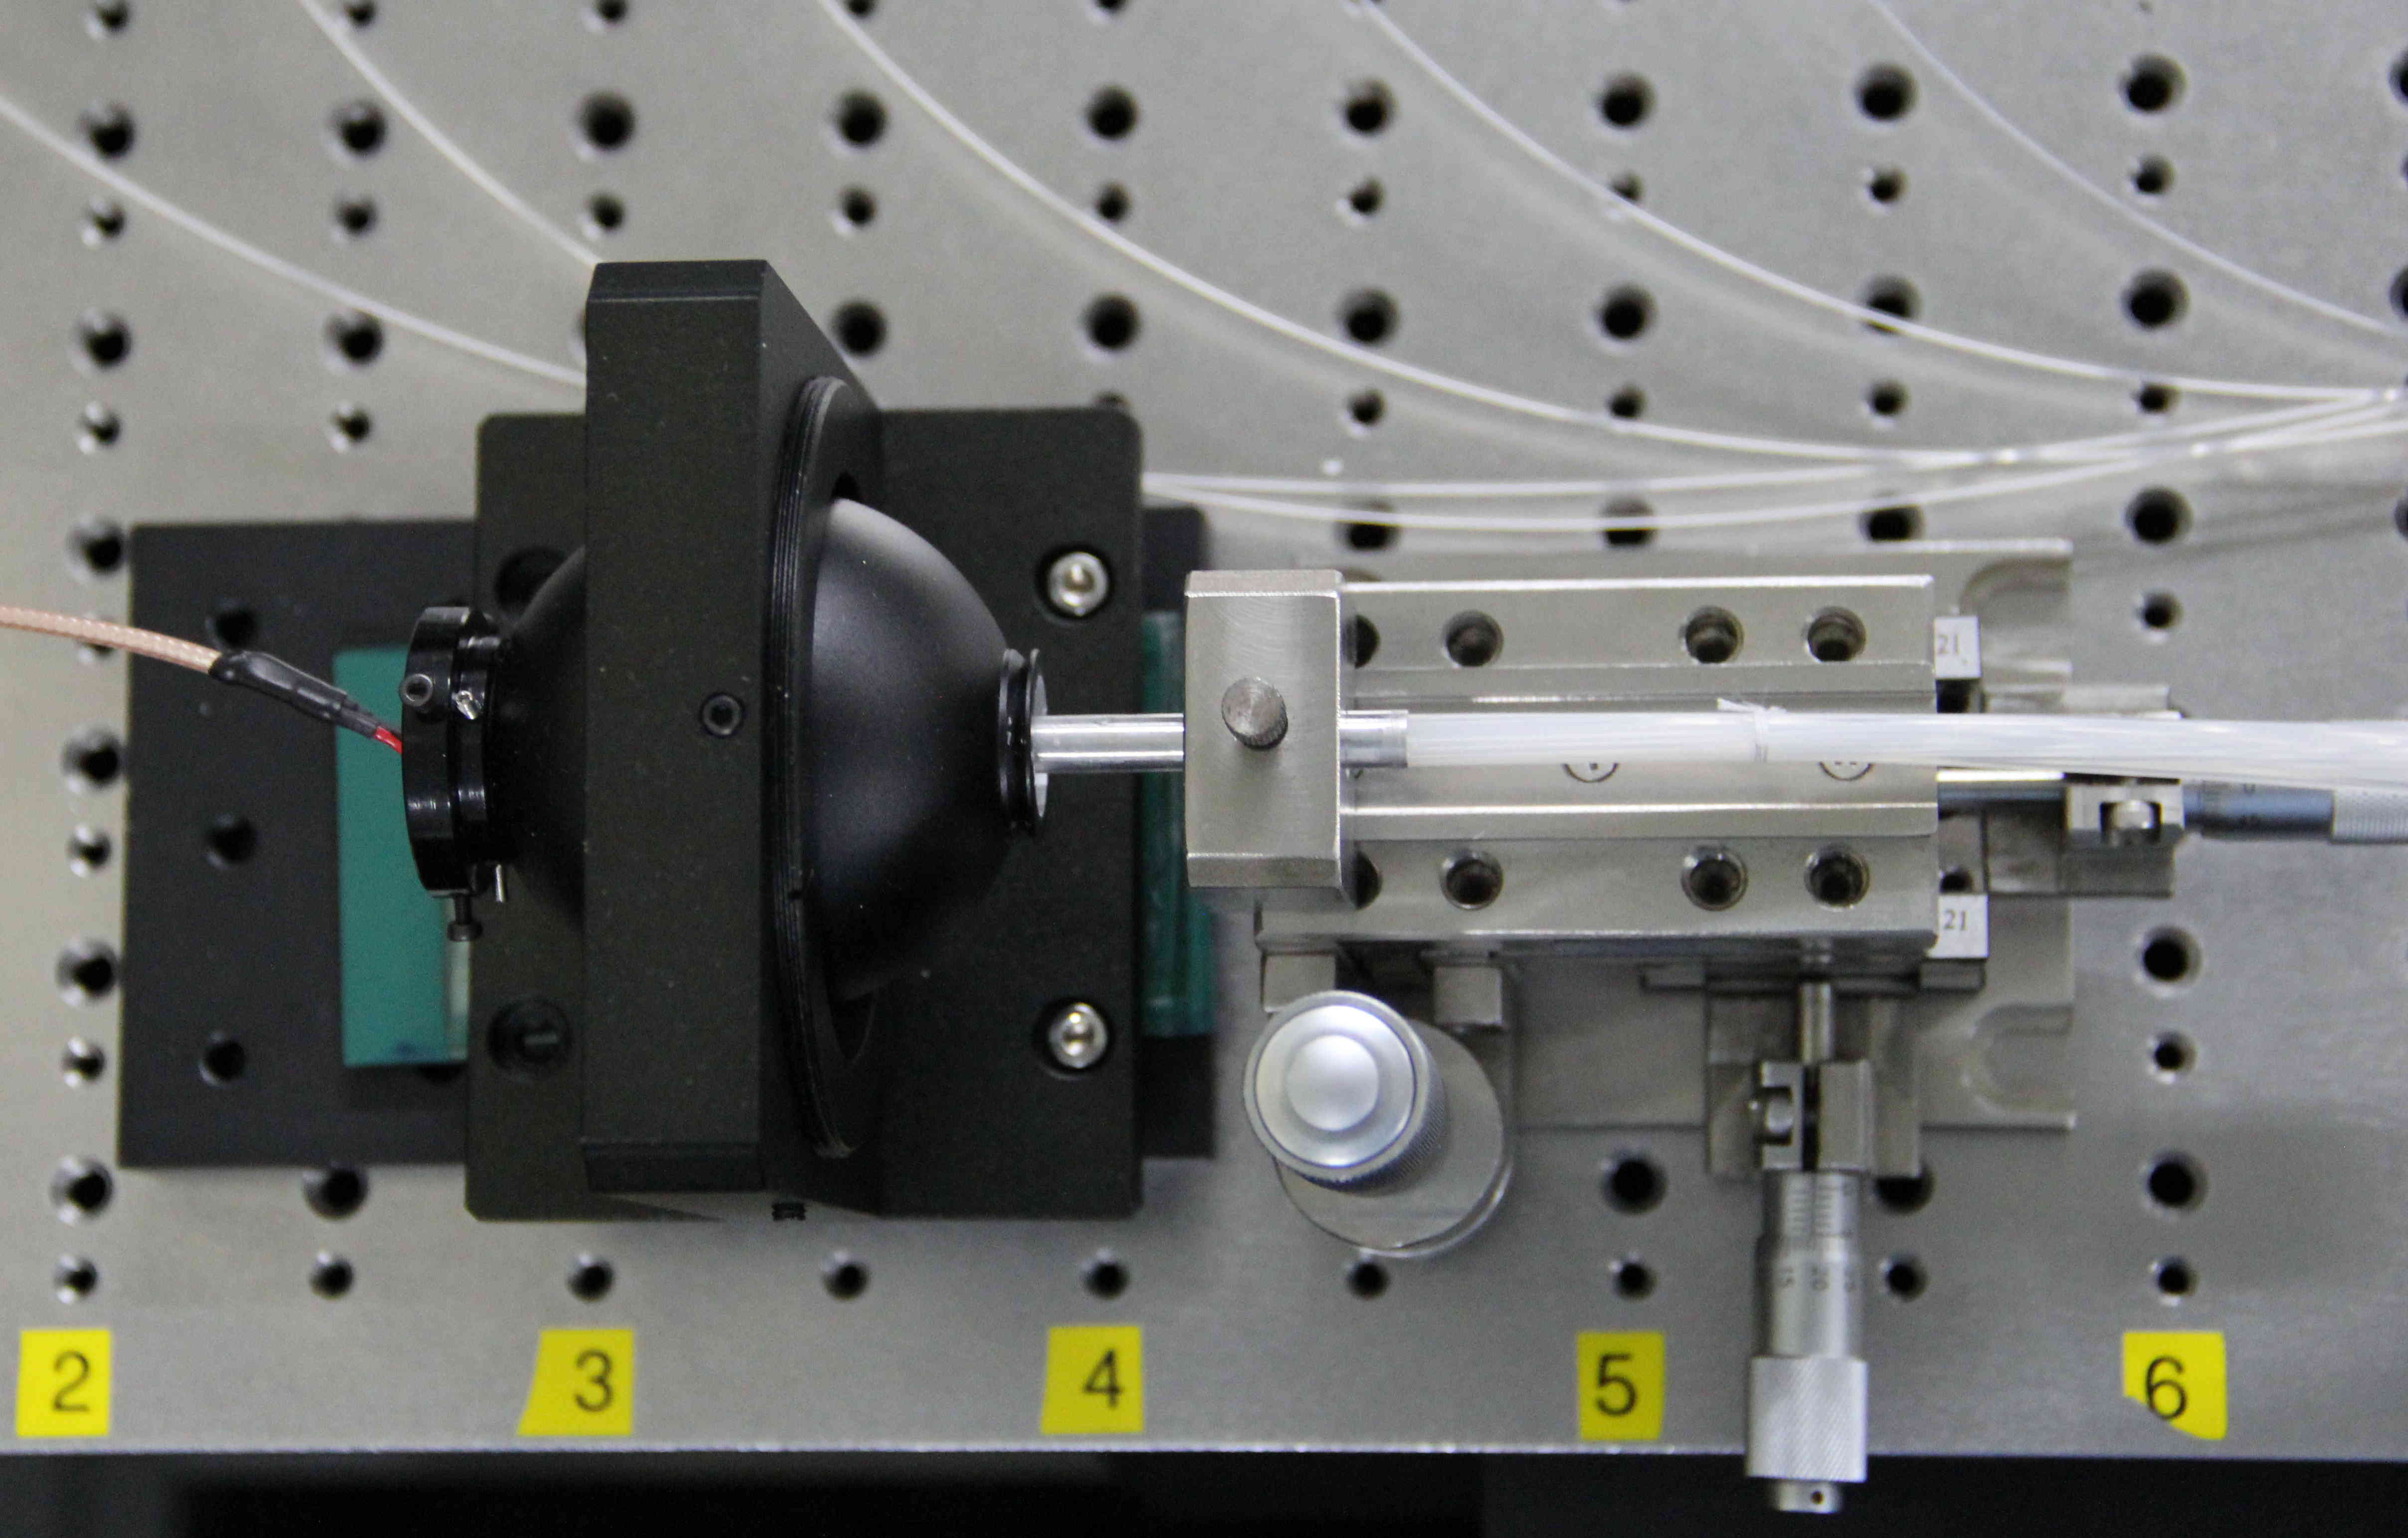
\includegraphics[width=90mm]{light_source1_crop}
\caption{Integration of the light distribution system as a whole}
\label{fig:light_source}
\end{figure} 

\subsection{Light Source}
\label{sec:light_source}

A high-power blue LED(\SI{3}{\watt}, \SIrange{465}{485}{\nano\meter}) coupled to a \SI{5}{\centi\meter} diameter integrating sphere is adoptted as the light source of the test bench.
The LED has been used previously in the monitoring and calibration system of Neutron Wall Detector at IMP~\cite{yuyuhong_led} and proved to be suitable for massive light distribution.
The integrating sphere~\cite{integrating_sphere}, which is painted interiorly with highly reflective material($\approx$\SI{98}{\percent} at \SI{400}{\nano\meter}), is used to convert the LED into a uniform light source.
To get better heat dissipation, the LED is fixed on a special designed base using thermally conductive silicone rubber(see Fig.\ref{fig:fibre_led_sphere}) and then coupled to the sphere directly, making the whole sphere as its heat sink.

An off the shelf hardware, Tektronix AFG3252 arbitrary/ function generator~\cite{afg3252}, is adpoted as the LED driver as well as the pulse generator.
AFG3252 has two analog outputs which can be synchronized together.
Thus one of them can be used for LED driving and the other one for DAQ triggering.
%Thus it be used as a trigger generator at the same time it driving the LED, which will symplify the DAQ configuration in most use cases. 
All the pulse parameters of AFG3252 can be adjusted in a wide range with high precison.% and an example is given in Fig.\ref{fig:afg3252_intensityVSvoltage}.
This is a critical feature for a test bench with an objective of versatiltiy, as diverse requirements for the light source exist for different applications.
An example of the light output of LED at various pulse parameters is shown in Fig.\ref{fig:afg3252_intensityVSvoltage}.
%As a commertial product, 
AFG3252 also possesses a rich set of hardware interfaces for remote control.
All these features make it an effective replacement of a dedicated LED driver. 
%After all, a stability better than \SI{0.5}{\percent} has been achieved after light intensity correction, the details of which will be given in Sec.\ref{sec:performance}.

Uniformity of the light source has been checked by using the same optical fibre to scan the the output port surface of the integrating sphere.
Light output at each position is readout by a Hamamastu R4443 Mod2 PMT and processed by the groud test electronics of DAMPE(see Sec.\ref{sec:application}). 
As shown in Fig.\ref{fig:uniformity_integratingsphere}, an uniformity within \textpm\SI{0.5}{\percent} has been reached.
This result makes the coupling between the light source and fibre bundle much easier and additional calibration for the spatial effect of the light source not needed. 

\begin{comment}
\begin{table}[h!]
\caption{Summary of AFG3252 Pulse Mode Characteristics}
\label{tab:afg3252}
 \begin{center}
 \begin{tabular}{lr}
 \multicolumn{2}{l}{Summary of AFG3252 pulse mode characteristics}\\ \hline
 Frequecny & max \SI{120}{\MHz} \\
 Amplitude & \SIrange{0}{5}{\volt} \\
           & resolution \SI{0.01}{\volt} \\
 Pulse width & min \SI{4}{\nano\second} \\
             & resolution \SI{10}{\pico\second} \\
 Leading edge & \SI{2.5}{\nano\second} to 0.625*pusle period \\
 Trailing edge & \SI{2.5}{\nano\second} to 0.625*pusle period \\
 %Jitter(typical) & \SI{100}{\pico\second} \\
 Interface     & GPIB, LAN, USB
 \end{tabular}
 \end{center}
\end{table} 
\end{comment}

\begin{comment}
One limitation of AFG3252 is that it has a limited leading edge of \SI{2.5}{ns}.
This may not be suitable for timing-related characterizations, where ultra-short(down to hundreds of \si{\pico\second} magnitude) light pulse is preferred.
In this case, a dedicated LED driver of special design(commertial or home-made)shall be used instead.
However the rich interfaces AFG3252 possesses still make it valuable as a trigger generator to control both the LED driver and DAQ remotely. 
\end{comment}

\subsection{Fibre Bundle}
\label{sec:fibre_bundle}

A bundle of 35(25 test channels, 2 reference channels and 13 spares) plastic clad silica fibres~\cite{optical_fibre} is utilized to distribute light to each PMT under test.
The fibres are \SI{1.5}{\meter} long and have a \SI{400}{\micro\meter} diameter core and a \SI{550}{\micro\meter} diameter cladding.
The numerical aperture(NA) is 0.37.
The relatively large core and NA make the fibre an efficient light extracter of integrating sphere output. 

For easier manipulation and to protect the fibres from mechanical stress, both ends of the fibre bundle are coated with stainless steel ferrules.
The bundle end is coupled to the centre of the output port of integrating sphere using a stable fibre alignment stage.
On the other end, each fibre is fixed using a customized fibre holder which allows two-dimensional position adjustment.
In each test run, fibres will be aligned to the centre of their corresponding PMT's cathode surface with a precision of \SI{0.5}{\milli\meter}.  

The light output of each fibre is measured after coupling the fibre bundle to the integrating sphere(see Fig.\ref{fig:light_source}).
The testing configuration is the same as the light source uniformity measurement except that an additional PMT is added to monitor the light intensity fluctuation of LED.
After the light intensity correction, a variance of \SI{10}{\percent} is observed among the fibres as shown in Fig.\ref{fig:fibre_diff}.
The result is a direct reflection of the light transmition difference among the fibres, as the contribution from light source non-uniformity is negligible.
Moreover, two light intensities of about 4 times difference have been used in this measurement and the result also shows no dependency on the light intensity. 
This is within expectation, because transmition coefficient is an intrinsic characteristic of the fibre itself.
Thus, transmition difference of fibres can be used as correction constants in the relative gain measurement described in Sec.\ref{sec:psd_gain}.
%%The testing configuration includes two R4443 Mode PMTs, one for light source monitoring and the other one for fibre testing.
%%As stable fixture for the tubes and fibres are utilitized, the major uncertainty comes from the coupling distance between the fibre and the PMT in the longitudinal direction.

%\begin{comment}


\begin{figure}
 \centering
 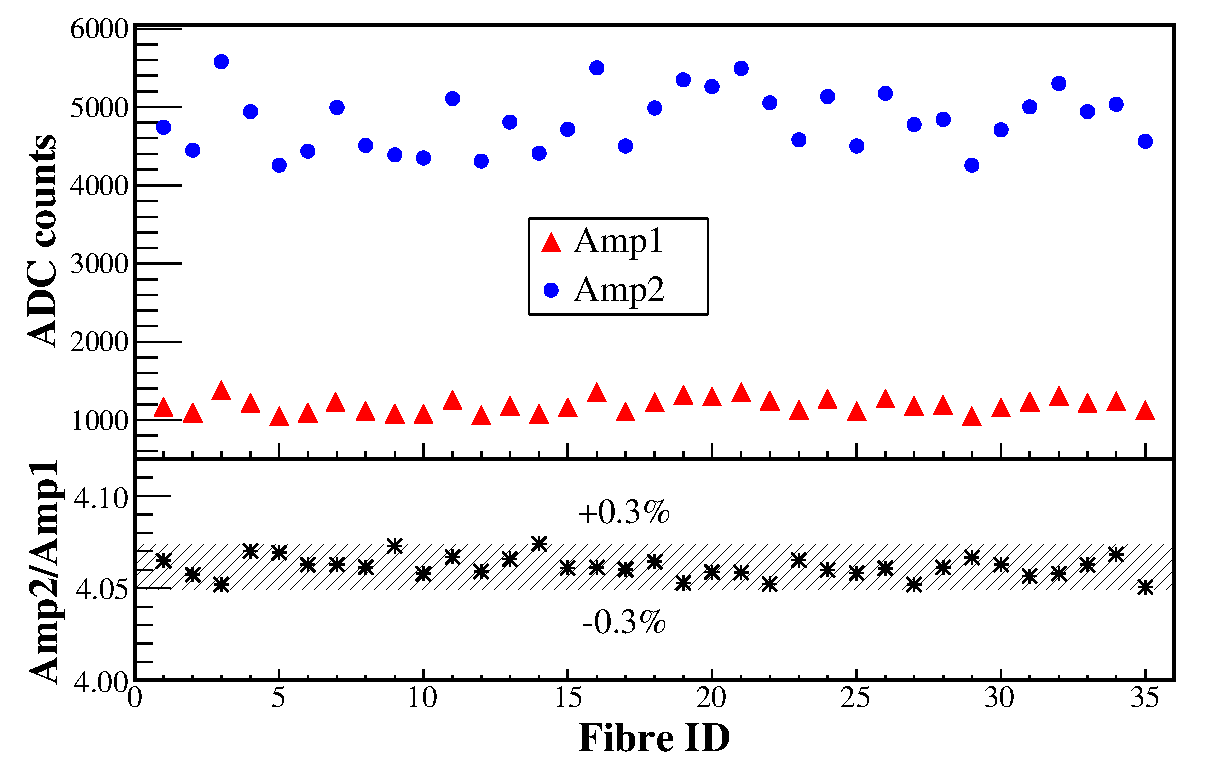
\includegraphics[width=90mm]{fibre_diff}
\caption{
Up: Light output uniformity of the fibre bundle measured at two light intensities.
Bottom: Ratio between the transmition difference measured at two light intesities, the results are consistent within \textpm\SI{0.3}{\percent}.}
\label{fig:fibre_diff}
\end{figure} 
%\end{comment}

\begin{figure*}
  \centering
 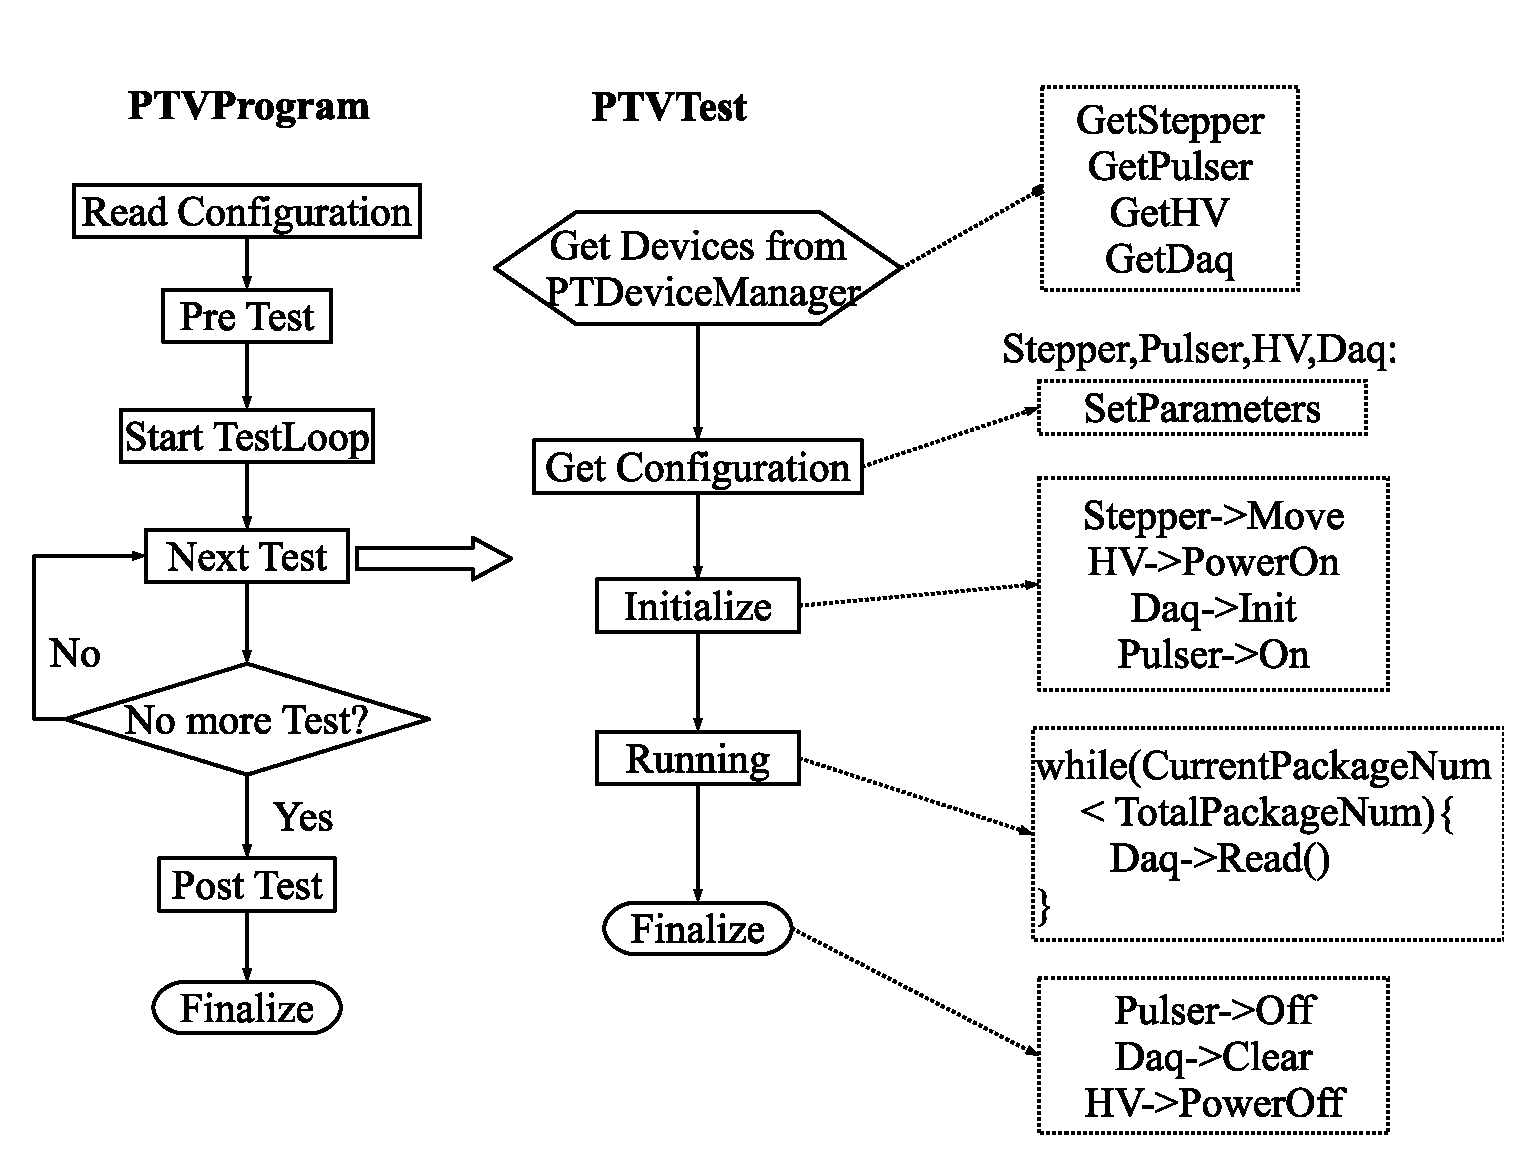
\includegraphics[width=130mm]{software_framework}
\caption{General PMT testing framework}
\label{fig:software_framework}
\end{figure*}


\begin{comment}
\subsection{Electronics and High Voltage Supply}
\label{sec:electronics}

A CAMAC system based on Wiener CC-USB control board has been set up for data acquisition.
This system is ready to use and shall be adequate for fast PMT characterization in daily use.
However, it shall be noted that the DAQ system of the test bench is expected to change frequently, as customized electronics with different control interface may be preferred in some project.

A mainframe from CAEN, SY1527LC, is adoptted as the high voltage supply system of the test bench.
While HV boards of various properties can be housed in SY1527LC, the same control interface will be used for all kinds of operation.
This feature simplifies our implementation of the test bench as a versatile equipment.More information about SY1527LC can be found in~\cite{sy1527lc}.
\end{comment}

%\FloatBarrier
%\begin{comment}
\begin{figure*}[t]
 \centering
 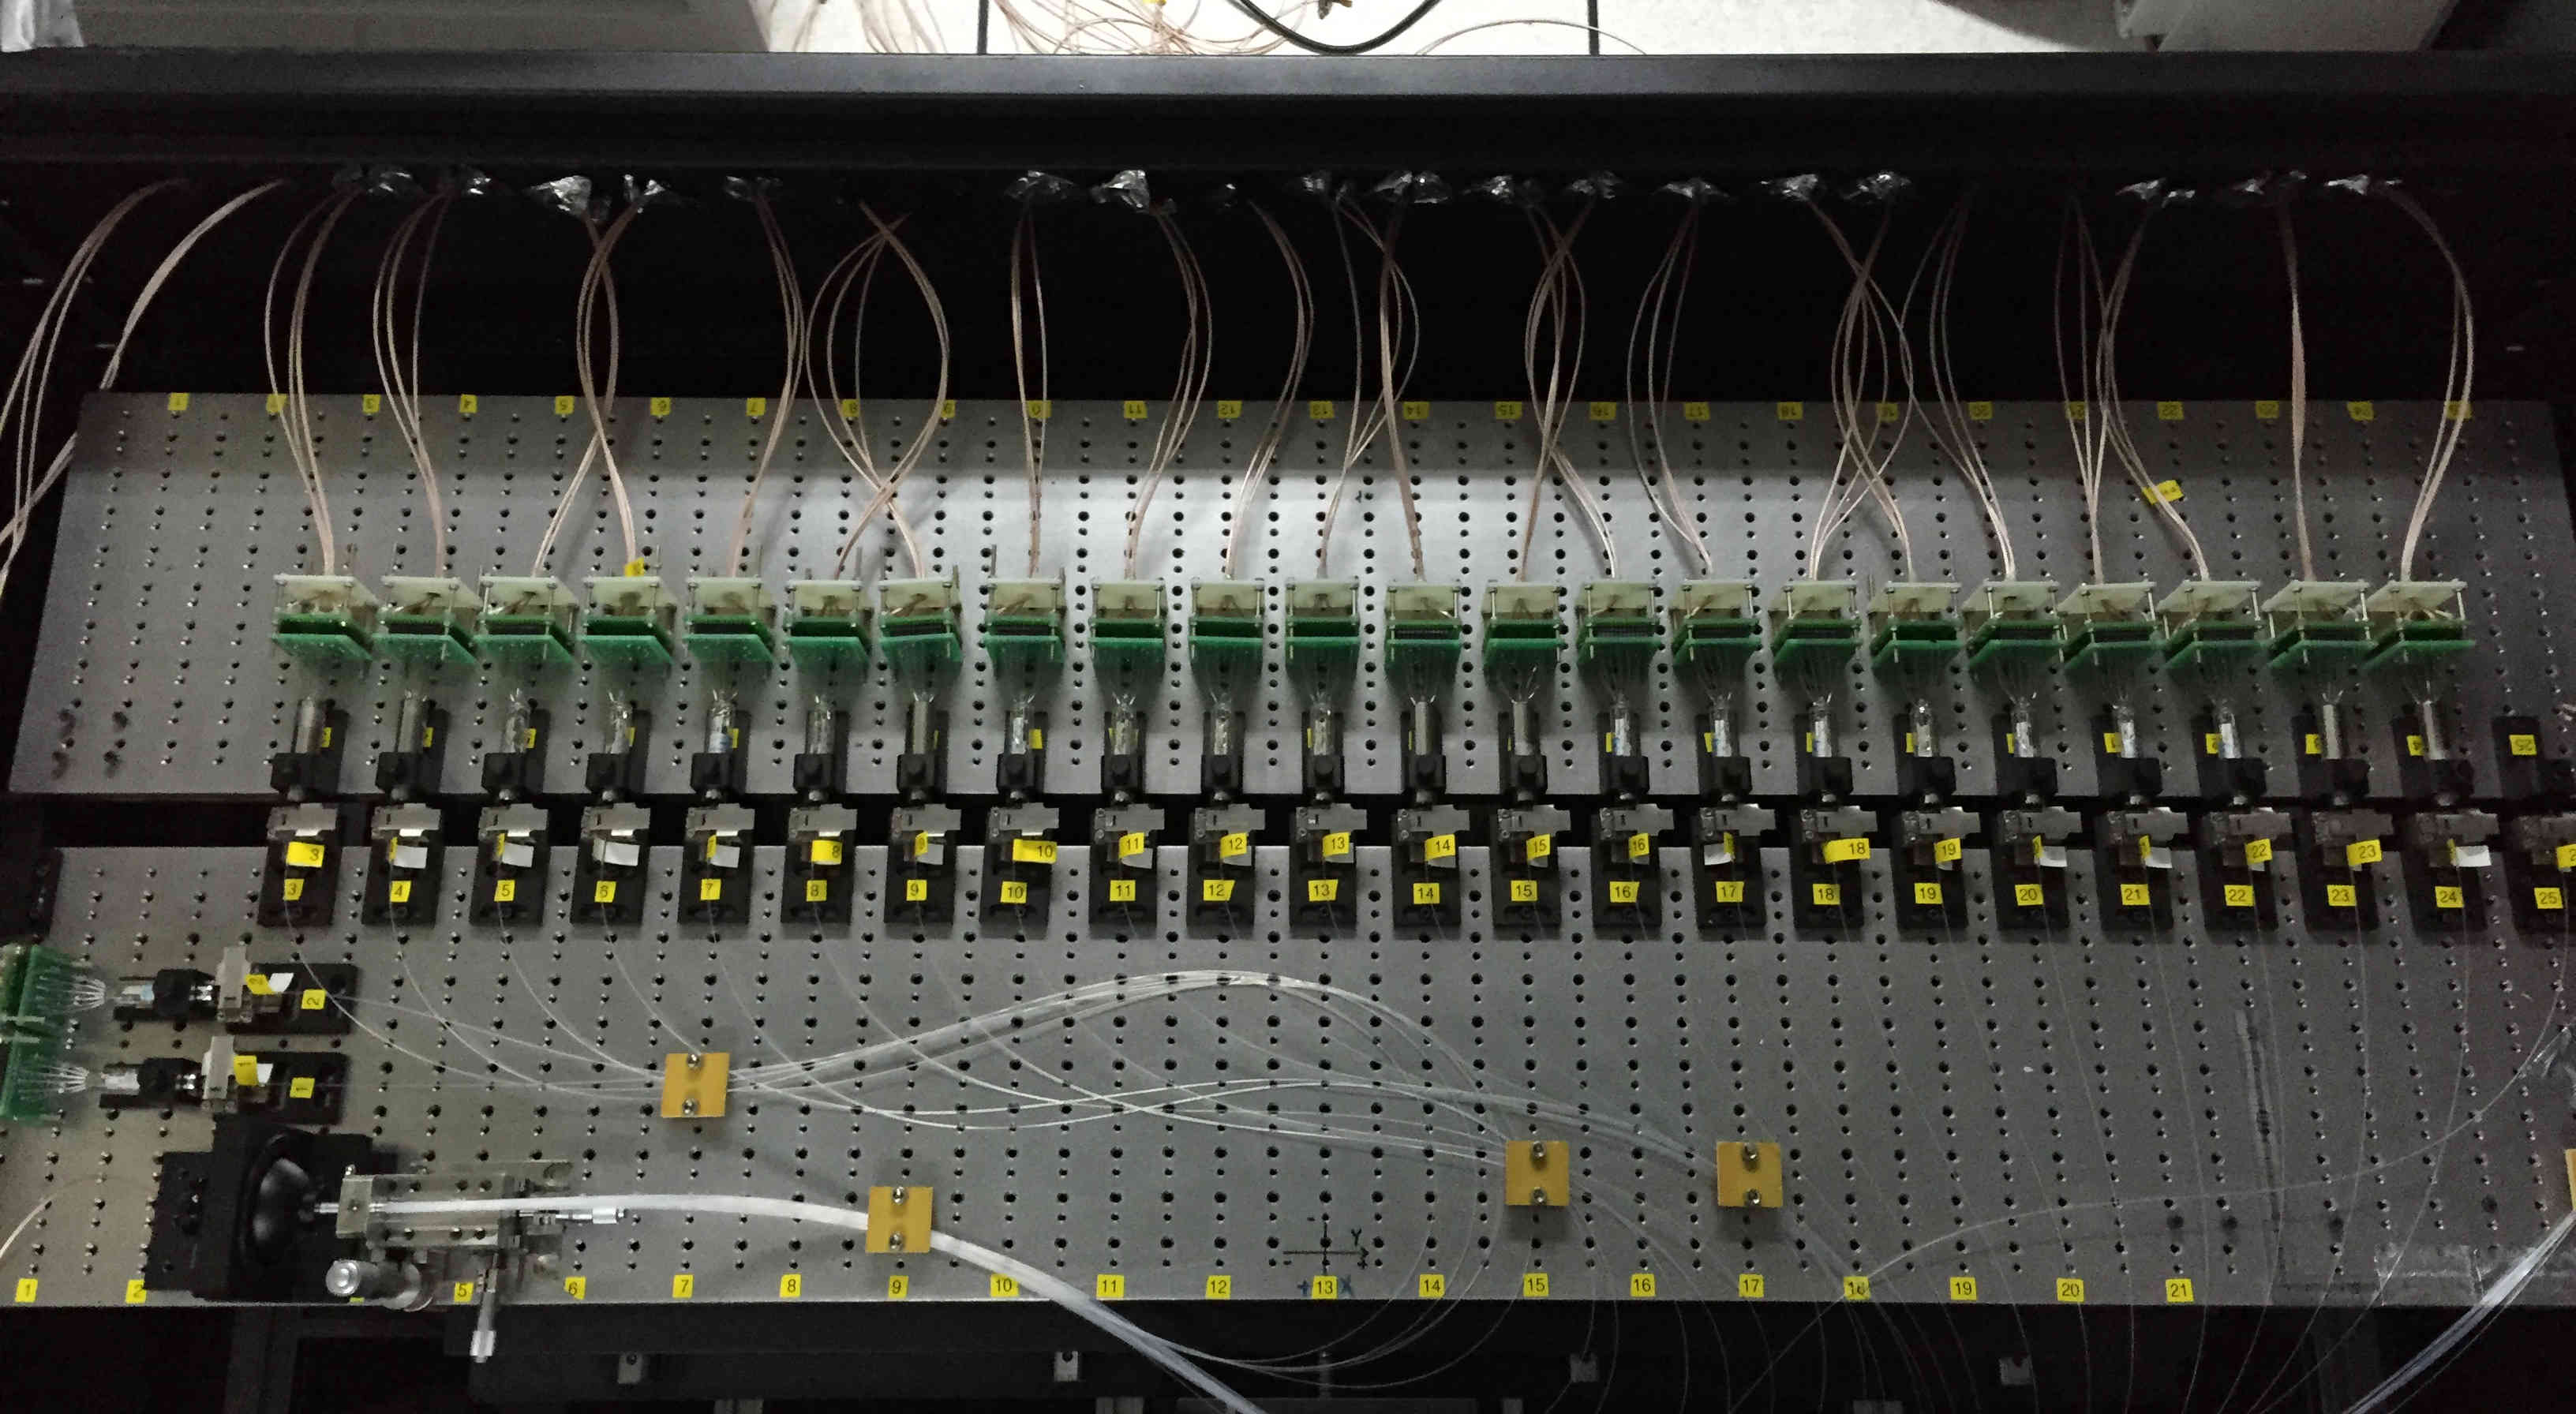
\includegraphics[width=130mm]{integration3}
\caption{Integration of all components of the test bench for R4443 Mod2 characterization.
Voltage dividers, same design as those used in the final assembly, are used. 
20 rare tubes are mounted and ready for test.
2 reference tubes can be seen in the bottom left corner of the picture. 
}
\label{fig:integrated_testbench}
\end{figure*}
%\end{comment}

\subsection{Software}
\label{sec:software}

The software system is a critical part of the test bench.
It is developped under Windows in C++ and divided into three hierarchies as follows:
\begin{enumerate}
 \item \textit{Device abstraction}, which not only serves as an interface to the underlying hardwares, but also handles the abstraction of different types of devices. 
 %which serves as an interface to the underlying hardwares.
 \item \textit{Framework libraries}, which defines a general testing pecedure and provides utility classes for configuration and management.
 \item \textit{User inerface}, which provides command line based or graphical executables for user interaction. 
\end{enumerate}

%Designed as a versatile equipment, different hardware modules may be used in the future.
Instead of developping a dedicated program each time a hardware changes, an abstraction of the devices is adoptted to separate the testing procedure from hardware implementation details. 
Abstract classes are defined for the four essential types of controlling device as shown in the rounded boxes in Fig.\ref{fig:testbench_overveiw}.
%Common operations of each type of device are extracted as the interface of the corresponding abstract class.
New hardware only needs to inherit from the corresponding abstract class and implement its interface methods and then registered in the singlton class \textit{PTDeviceManager}, leaving all other part of the software unchanged.
Currently, concrete device classes for the hardware described in this section have all been implemented and fully tested.
%Used concrete device class shall be registered in the singlton class \textit{PTDeviceManager} and retrieved from it in other part of the software. 

Built upon the abstract device inerface, a general testing framework is defined as shown in Fig.\ref{fig:software_framework}.
%As a first step, all used concrete device classes shall be registered in the singlton class \textit{PTDeviceManager}.
%Devices are then retrieved from \textit{PTDeviceManager} in all other part of the software.
%Testing procedures are grouped as shown in Fig.\ref{fig:software_framework}.
\textit{PTVProgram} represents the measurement for a specific characteristic of PMT, such as cathode uniformity, gain and so on.
\textit{PTVTest} is a subunit of \textit{PTVProgram}, which encapsulates the real device operations performed under a specific condition.
%As an example, typical implementation for \textit{PTVTest} using fake code is presented in the third column of Fig.\ref{fig:software_framework}.
A \textit{PTVProgram} may consist of a series of \textit{PTVTest}s, which are invoked sequentially in a test loop.
For example, in cathode uniformity measurement, the stepping motor will move to a series of positions and the PMT response will be recorded by the DAQ at each position.
Here, device operations performed at each position constitute a \textit{PTVTest} and tests at all positions constitute a \textit{PTVProgram}.
Additional operations may be added in the \textit{PreTest} and \textit{PostTest} methods of \textit{PTVProgram}, which will be invoked before and after the test loop repectively.
Typically, PMT warming can be performed in \textit{PreTest} and analysis can be done in \textit{PostTest}.
\textit{PTVProgram}s of various testing objectives will finally be chained together to constitute a complete characterization of PMT.

Finally, a light-weight user interface based on PDCurses~\cite{pdcurses} has been developped.
This program features in device control, status monitoring and information logging.
Thanks to the abstraction described above, the architecture of the program is rather independent of the specific hardware used and testing program performed.
A decoding function from binary file to root file~\cite{root} is also incorporated into it for online monitoring.
However, more detailed analysis are considered project specific and not included in the program. 

\section{Application in the PMT testing for PSD of DAMPE}
\label{sec:application}

PSD adopts Hamamastu R4443 Mod2~\cite{r4443_mod2} for scintillation light detection.
%R4443 Mod2 is a \SI{14.5}{\milli\meter} diameter, 10 stages photomultiplier tube with a minimum photocathode area of about \SI{10}{\milli\meter}.  
R4443 Mod2 is a ruggedized and low noise bialkali photocathode version of the previous R4443 tube, which is suitable for space usage. 
To cover the large dynamic range required by PSD, both dynode5 and dynode8 of R4443 Mod2 are readout by a customized voltage divider.
Signals are then processed by a highly-sensitive ASIC chip(VA160~\cite{va160}) with a linear range of \SIrange{0}{12}{\pico\coulomb} and digitized by an ADC with 14~bits resolution.
Both the gain of dynode8 and the ratio between the gain of dynode8 and dynode5 need to be ajusted carefully to accommodate the input range of VA160 as well as to obtain a \SI{25}{\percent} energy response uniformity among all detection units of PSD.

Concrete \textit{PTVProgram}s for gain measurement, dynode8/ dynode5 ratio measurement and cathode uniformity measurement have been implemented for R4443 Mod2 characterization.
%Commertial QDC of CAMAC system features an input range of several hundreds \SI{}{\pico\coulomb} and thus is not suitable for data acquisition in this application.
On the other hand, commertial electronics of CAMAC system are not suitable for signal processing in this application as they features an input range of several hundreds \SI{}{\pico\coulomb}.
To obtain more realistic results, the standalone front-end electronics(FEE) and DAQ board for PSD groud test, which are based on the same design as the flight model except that commertial grade components are used, are utilitized.
%The FEE is based on the same design as the flight model except that commertial grade components are used.
Dedicated \textit{PTVDaq} based on NI-VISA library has been implemented for this specific system.

A typical test run for R4443 Mod2 characterization takes about 5 hours including 2 hour's PMT warming time.
About 20 tubes are mounted and tested in a single test run, as shown in Fig.\ref{fig:integrated_testbench}.
Totally, 28 test runs were performed in a period of about one month.
570 rare R4443 Mod2 tubes have been charaterized and 196 of them were selected for production and qualification.
The final analysis results are stored in a MySQL database for convenient query.

Selection of tubes based the test data is not the object of this article.
Here, only the major results are presented with a focus on the demonstration of the validity of the test bench. 

\subsection{Gain of Dynode8}
\label{sec:psd_gain}

%\begin{comment}
\begin{figure}[h!]
 \centering
 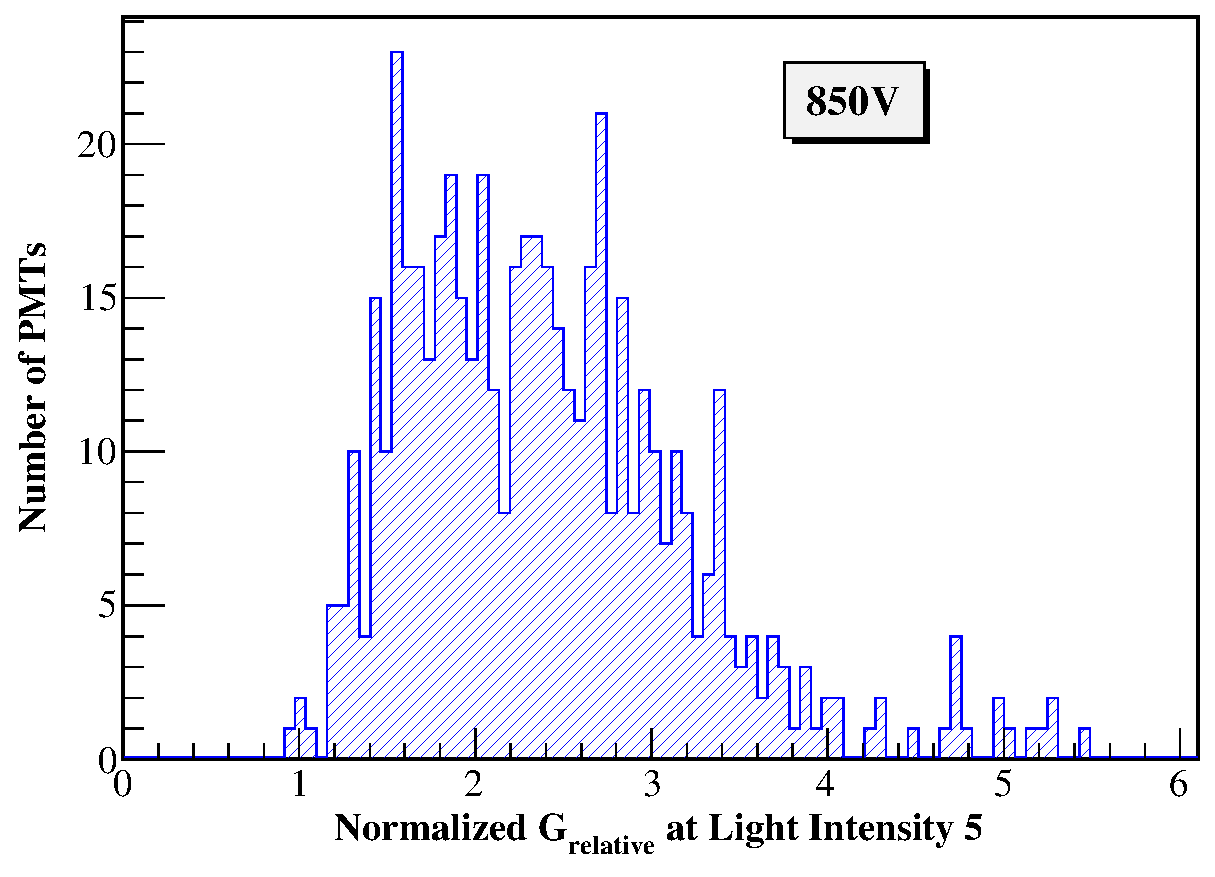
\includegraphics[width=85mm]{GainDist}
\caption{Relative gain distribution at 850V measured using light intensity 5.
Data are normalized to a specific tube of small gain.}
\label{fig:gain_dist}
%\end{figure}
%\end{comment}
\vspace*{0.1in}
%\begin{figure}[H]
 \centering
 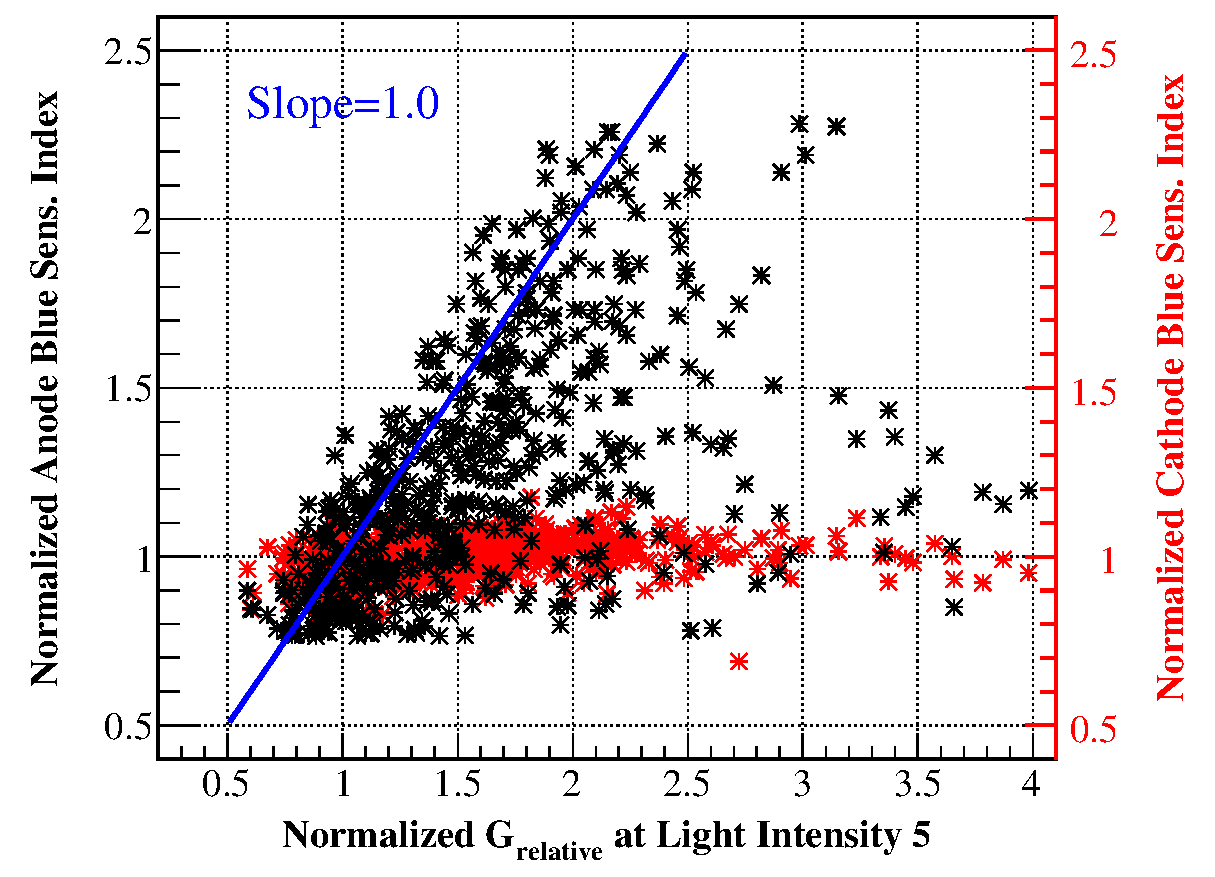
\includegraphics[width=85mm]{correlation_new}
\caption{Correlation between the parameters given by Hamamastu and the gain measured using the test bench.
Data are normalized to the same tube.}
\label{fig:gain_correlation}
\end{figure} 
%\end{comment}

The gain of dynode8 is measured by recording the response of PMT at a fixed light source setting. 
This is a relative method and the result depends on the light intensity used:
\begin{equation}
 G_{relative} = L_i \times G(V) = L_i k V^\beta
\end{equation}
where $G(V)$ is the absolute gain of PMT and $L_i$ is the light intensity at a specific light source setting.
$G_{relative}$ is a direct reflection of $G(V)$ if the inconsistency of light intensity can be eliminated.
Two corrections are made to accomplish this goal, as follows: 
\begin{equation}
 G_{relative} = \frac{A_{Mean}}{K_{RunID} T_{ChID}}
\end{equation} 
where $A_{Mean}$ is the mean value of the raw ADC spectrum at the specified light source setting,
$K_{RunID}$ is the light intensity fluctuation of LED between different test runs and $T_{ChID}$ is the light transmition difference among fibres of different testing channels.
$K_{RunID}$ can be calculated at each test run using the reference PMT.
$T_{ChID}$ is a constant parameter, which has been measured accurately before(Sec.\ref{sec:fibre_bundle}).
These corrections are made for all measurement results.

5 light source settings, with a maximum intensity difference of about 2 times, have been used for relative gain measurement.
The results from different light intensities are cross checked and they are consistent with each other.
Distribution of the relative gain at 850V is shown in Fig.\ref{fig:gain_dist}, where all tubes are normalized a specific tube of relatively small gain. 
A maximum of about 6 times difference in the gain has been observed.

7 voltage steps, from \SIrange{700}{1000}{\volt} with a \SI{50}{\volt} step, are scanned to measure the gain variation as a function of supply voltage.
The results are then fitted using power law function.
Based on the fitting result,the gain at the Hamamastu equivalent voltage is calculated for comparison with the parameters on the data sheets provided by Hamamastu.
Hamamastu equivalent voltage is the voltage that should be applied to the PSD voltage divider so that the same voltage on dynode 8 can be achieved as that used by Hamamastu for PMT testing.
Linear correlation between the calculated gain and the anode blue sensitivity index has been observed, while no relation to the cathode blue sensitivity has been found(see Fig.\ref{fig:gain_correlation}).
This result is a direct demonstration of the validity of our testing method.


\begin{figure}
 \centering
 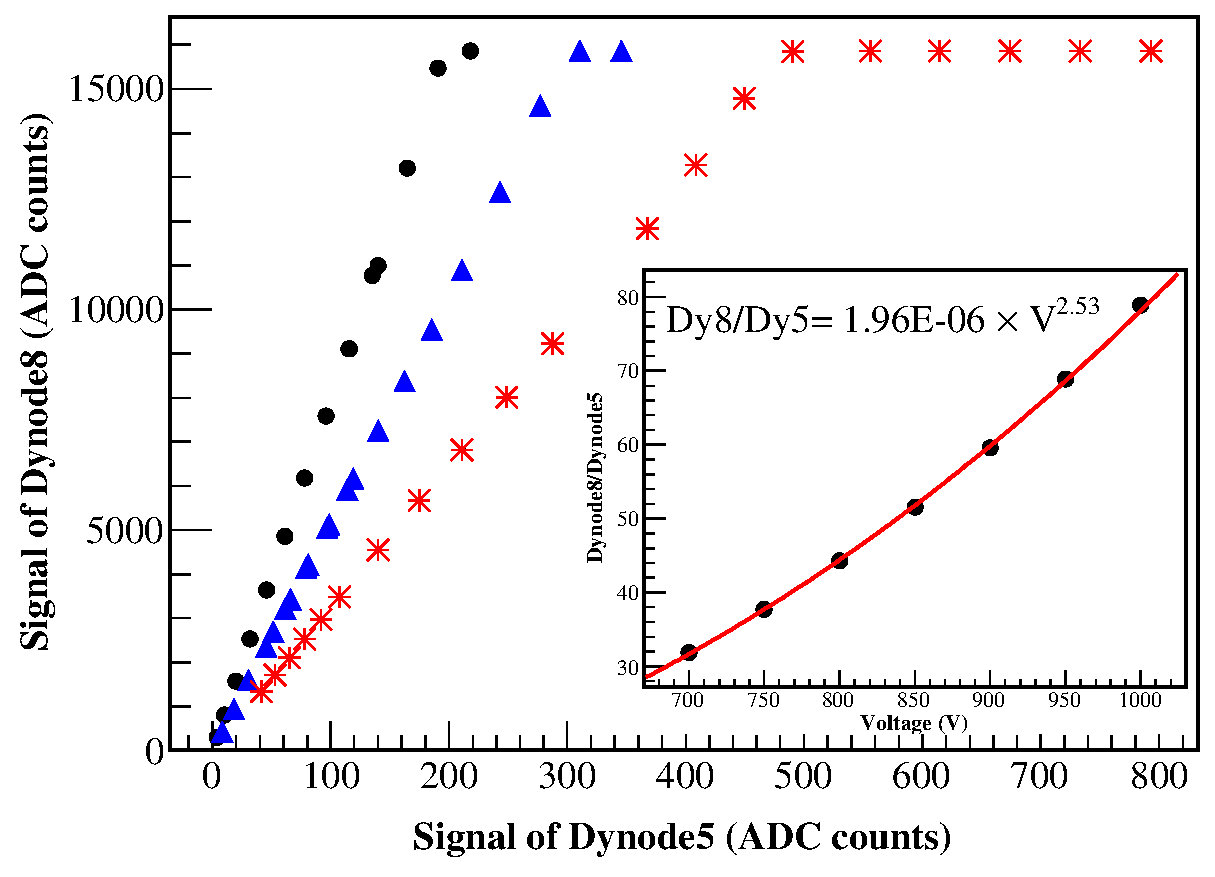
\includegraphics[width=90mm]{dy58_example}
\caption{Example of the measurement of dynode8/dynode5.
Correlation between dynode5 and dynode8 at 1000V, 850V and 700V is presented for a typical tube.
Power law fit to the measured dynode8/dynode5 at 7 voltage steps is shown in the inset graph.
}
\label{fig:dy58_example}
\end{figure} 

\begin{figure}
 \centering
 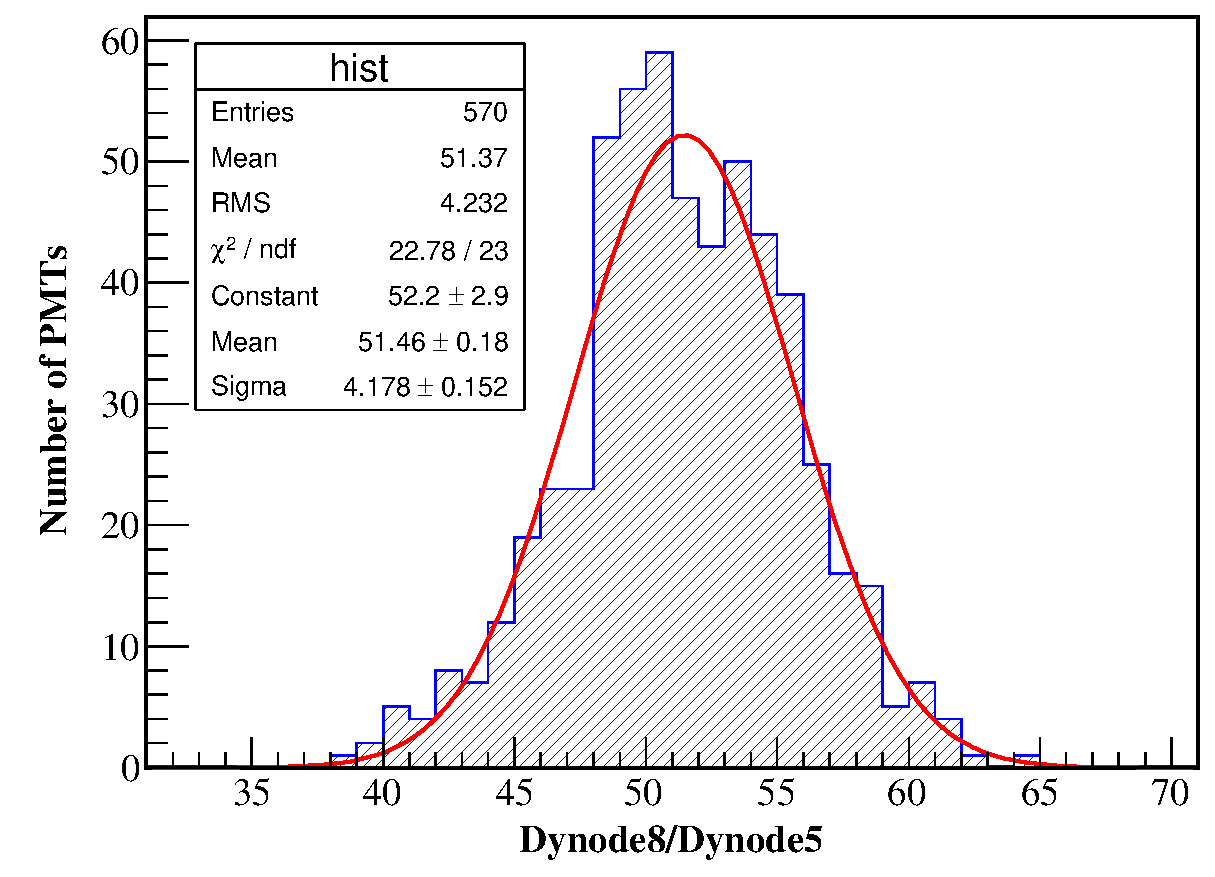
\includegraphics[width=90mm]{dy58_dist}
\caption{Distribution of the Dynode8/Dynode5 at the Hamamastu equivalent voltage.}
\label{fig:dy58_dist}
\end{figure} 

\begin{figure*}
 \centering
 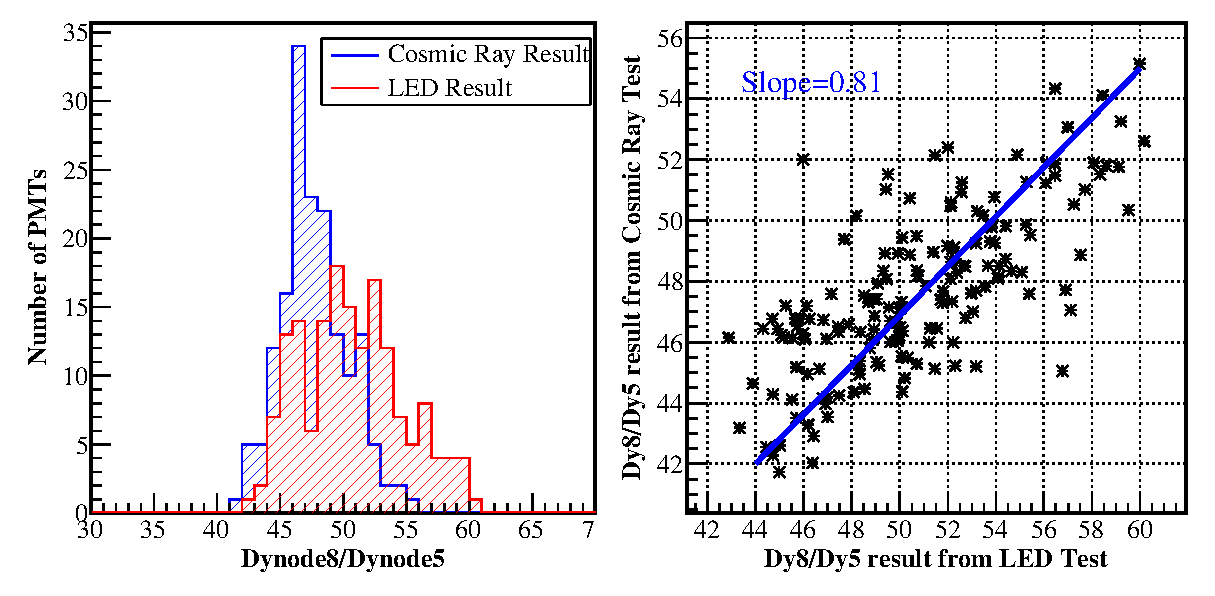
\includegraphics[width=140mm]{dy58_ledvscm}
\caption{Comparison of the dynode8/dynode5 result measured using LED and using cosmic ray.
Same voltage divider and voltage value are utilitized in these two measurements.}
\label{fig:dy58_ledvscm}
\end{figure*} 


\subsection{Ratio between the Gain of Dynode8 and Dynode5}
\label{sec:psd_dy58}

The ratio between the gain of dynode8 and dynode5 is measured by varying the light intensity in a large range until saturation of dynode8 singal is observed, as shown in Fig\ref{fig:dy58_example}.
The same procedure is repeated at 7 voltage steps, from \SIrange{700}{1000}{\volt} with a \SI{50}{\volt} step, to obtain the dynode8/dynode5 dependency on voltage.
As with the gain of dynode8, the dependency can be fitted accurately with a power law function, as shown in the inset graph of Fig.\ref{fig:dy58_example}.
The ratio between the gain of dynode8 and dynode5 can then be calculated at any voltage value based on the fitting result.
As an example, the distribution of dynode8/dynode5 ratios at the Hamamastu equivalent voltage is shown in Fig.\ref{fig:dy58_dist}.
The variance is much smaller than that of gain.

Matching between the result measured using the test bench and the result measured using comsic ray after coupling to the plastic scintillator strip of PSD has been checked for a small sample of tubes.
As shown in Fig.\ref{fig:dy58_ledvscm}, a small shift of the mean value exists and the distribution of cosmic ray test is narrower than that of LED test. 
This effect may be attributed to the fact that in cosmic ray test the result is an average of the response in the whole cathode surface, while in LED test the result is the reponse at the center of the cathode surface with a spot of \SI{1}{\milli\meter}.


\subsection{Cathode Uniformity}
\label{sec:psd_cathodescan}

%\begin{comment}
\begin{figure}
 \centering
 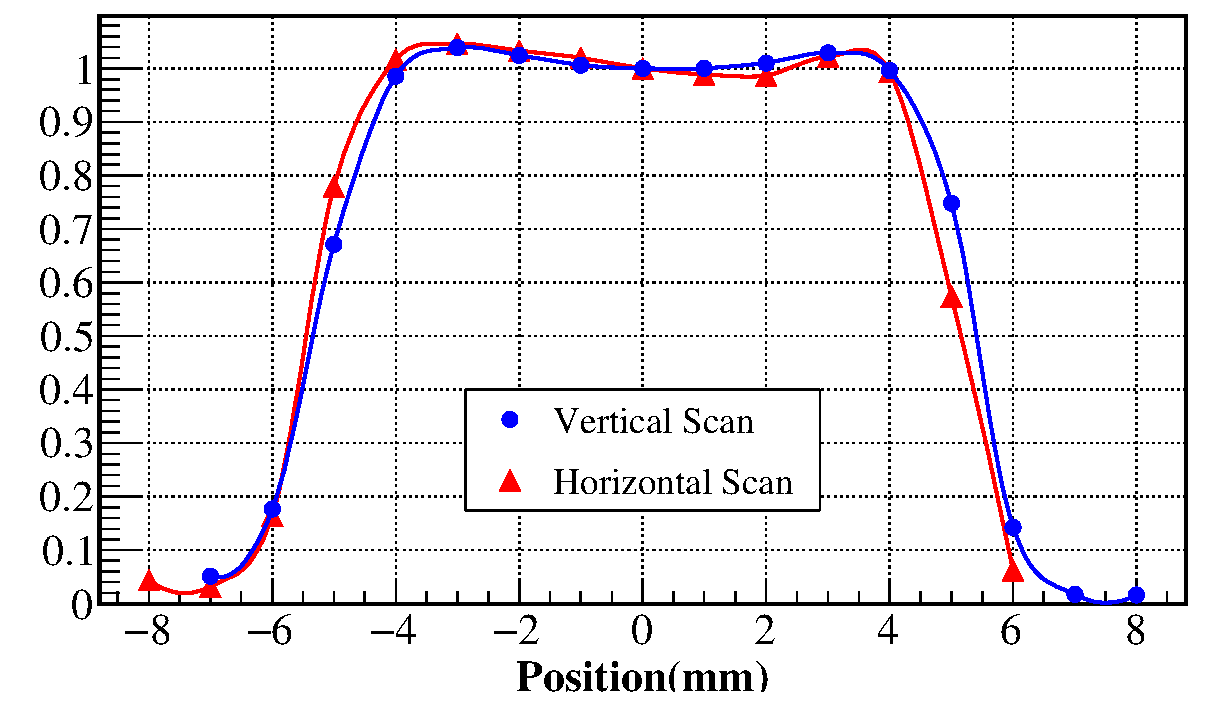
\includegraphics[width=90mm]{cathode_uniformity}
\caption{A typical cathode uniformity of R4443 Mod2.
Relative gain at each position is normalized to the center of the input window.}
\label{fig:cathode_uniformity}
\end{figure} 

%\end{comment}

%A \textit{PTVProgram} for cathode uniformity characterization is implemented to validate the position scanning ability of the test bench.
Cathode uniformity is measured by scanning the input window of R4443 Mod2 both in the verical and horizontal direction with a step of \SI{1}{\milli\meter}.
At each position, the relative gain is measured at a fixed light source setting according to the method described in Sec.\ref{sec:psd_gain}.
A typical result is shown in Fig.\ref{fig:cathode_uniformity}.

Cathode uniformity of 20 sample tubes have been measured in a single test run.
Measurement results of all these tubes are summarized and it is found that in the central \SI{9}{\milli\meter} of the photocathode, about \SI{75}{\percent} of the testing data are within \textpm\SI{10}{\percent} range around each tube's average value.
R4443 Mod2 has a photocathode with a minimum effective area of about \SI{10}{\milli\meter}.

\section{Summary}
\label{sec:summary}

Performance of the test bench can be extracted from the reference PMTs using the data obtained in the PMT characterization for DAMPE PSD.

As a first step, stability of the reference PMT configuration is checked.
The response of the two reference PMTs to various light intensities is linearly correlated.
An example is given in Fig.\ref{fig:refgain_relation}, where the data points can be fitted quite well with linear function.
Slope $M$ of the fitting function does not depends on the light intensities used as follows:
\begin{equation}
 M = \frac{G_{ref1} T_{ref1}}{G_{ref2} T_{ref2}}
\end{equation}
where $G_{ref}$ is the absolute gain of each reference PMT and $T_{ref}$ is the transmition difference of fibres between reference channels.
As $T_{ref}$ is a constant parameter, $M$ is only related to the gain difference between the reference PMTs.
$M$ values are calculated for all test runs and the variance of it is found to be \SI{0.48}{\percent}.
The samll variation verifies the high stability of the reference PMTs.

\begin{figure}[h!]
 \centering
 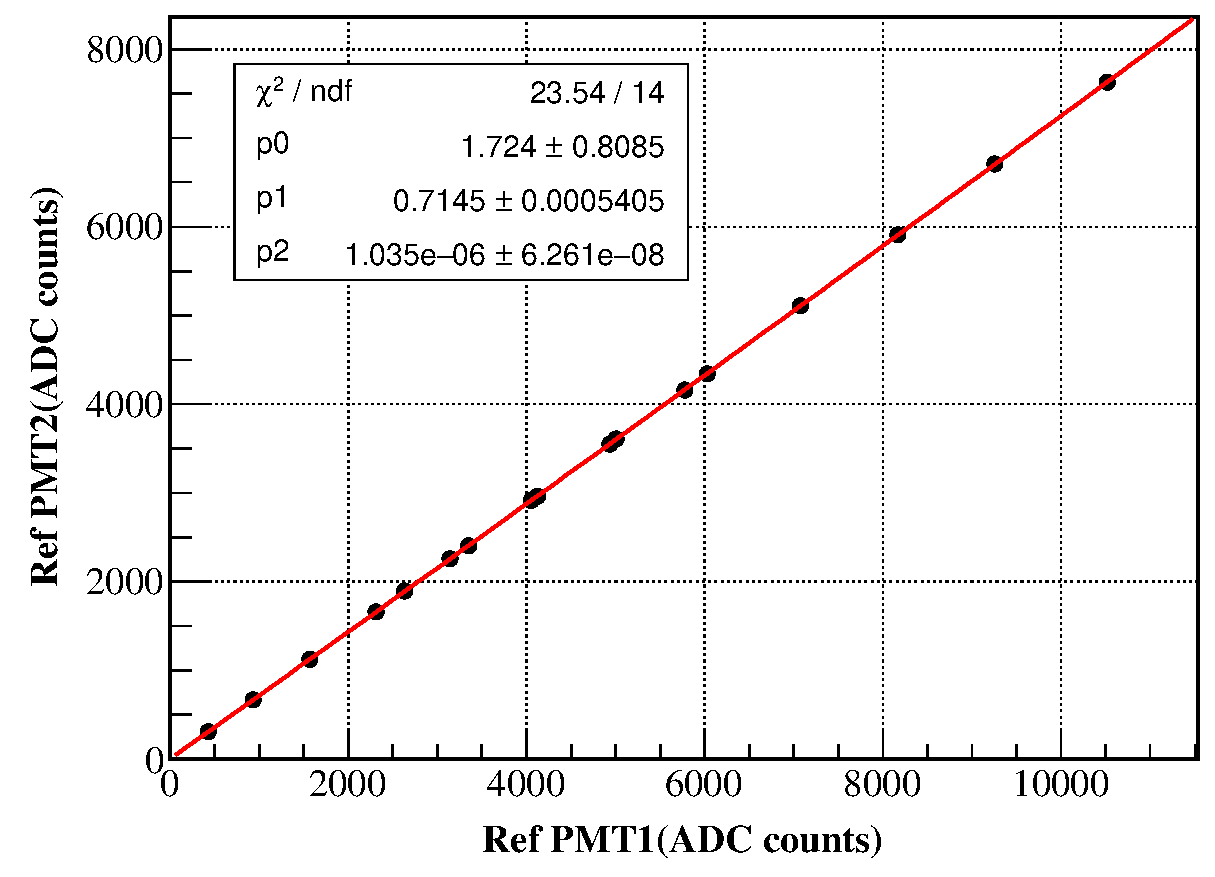
\includegraphics[width=90mm]{RelativeGainRef}
\caption{Correlation of the responses to various light intensities between the two reference PMTs measured at 900V.}
\label{fig:refgain_relation}
\end{figure} 

%\begin{comment}
\begin{figure}[H]
 \centering
 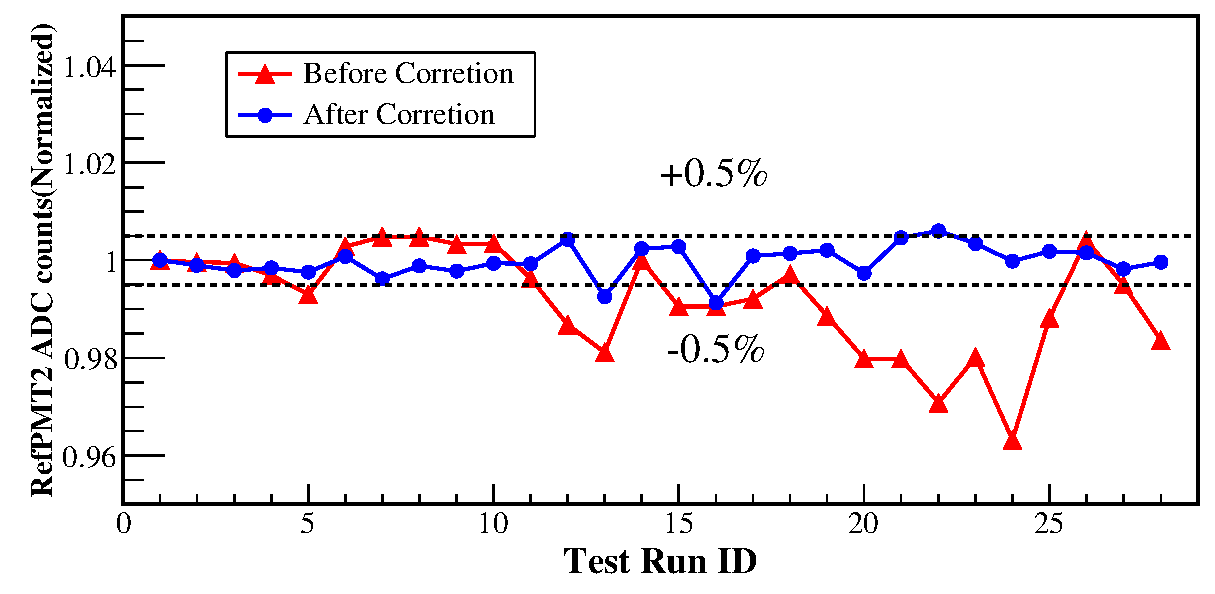
\includegraphics[width=90mm]{led_stability}
\caption{Stability of the light source monitored by Reference PMT2 at 900V.
The data corresponds to a period of about one month and is all scaled to the first test run.
Red Triangle: mean value of raw ADC counts, recorded at the same light source setting before light intensity correction.
Blue Circle: relative gain, measured after using Reference PMT1 for light intensity correction.}
\label{fig:led_stability}
\end{figure} 

\begin{figure}[H]
 \centering
 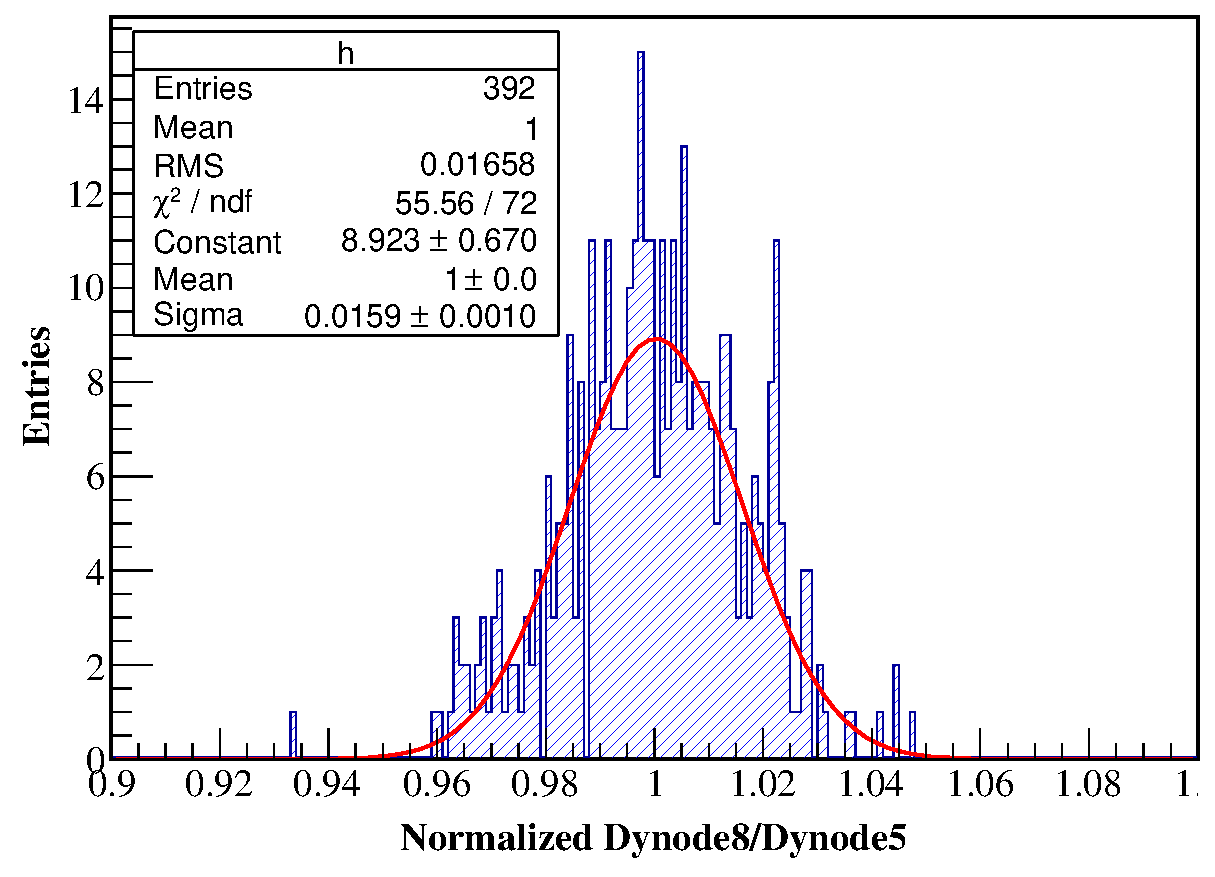
\includegraphics[width=90mm]{RefDy58Dist}
\caption{Distribution of the ration between dynode8 and dynode5 of the reference PMTs measured by the test bench.
Results from all voltage steps are normalized to their respective mean value of all test runs.}
\label{fig:dy58_stabiltiy}
\end{figure} 
%\end{comment}

By investigating the response of the reference PMT to a fixed light source setting, a maximum variation of \SI{4}{\percent} in the light intensity of LED is observed during a period of about one month.
Light intensity fluctuation can be corrected using the method described in \ref{sec:psd_gain}.
As two reference PMTs exists, this method can be validated by using one of them for correction and then checking the relative gain of the other. 
The result is shown in Fig.\ref{fig:led_stability}.
After light intensity correction, stability of the light source is controlled within \textpm\SI{0.5}{\percent}.


Reference PMTs underwent the same testing procedures as tubes under test.
Thus, spread of the distribution of the parameters of reference PMT is an indication of the uncertainty of the testing method.
As an example, distribution of the ratio between dynode8 and dynode5 of the reference PMTs is shown in Fig.\ref{fig:dy58_stabiltiy}, where the results from different voltage steps are normalized to their respective mean value of all test runs and filled together.
The variance is \SI{1.59}{\percent}, which is adoptted as the testing uncertainty of the dynode8/dynode5 measurement.
%%As an example, dynode8/dynode5 of the reference PMTs at a fixed voltage are first scaled to their mean value of all test runs.
%%Then, scaled value at all voltage steps are filled into the histogram as shown in Fig.\ref{fig:dy58_stabiltiy}.
%%The variance of the distribution is \SI{1.59}{\percent}, which is adoptted as the testing uncertainty of the dynode8/dynode5 measurement.
In the same way, the uncertainty in the measurement of relative gain is estimated to be \SI{0.53}{\percent}. 

These results have all validated the high stability of the test bench system.
Considering the flexible and open platform it possesses, the test bench is suitable for fast PMT characterization in other experiments. 

\begin{comment}
%%%%%%%%%%%%%%%%  Conclustion   %%%%%%%%%%%%%%%%%%%%%%%
\section{Conclusions}
\label{sec:conclustions}

We bulilt a dedicated test bench for massive PMT characterization, which is suitable for various testing configurations.
Initial application of the test bench in DAMPE PSD has proved the effectiveness of the test bench.
Thus, it is adoptted as a standard laboratoy equipment for daily use at IMP.

\end{comment}
%%%%%%%%%%%%%%%% Acknowledgement %%%%%%%%%%%%%%%%%%%%%%%
\section*{Acknowledgement}

This work was supported by the Strategic Priority Research Program on Space Science of the Chinese Academy of Science, Grant No. XDA04040202- 3. 
%%%%%%%%%%%%%%%%    Appendix     %%%%%%%%%%%%%%%%%%%%%%%
%% The Appendices part is started with the command \appendix;
%% appendix sections are then done as normal sections
%\appendix
%\section{}
%\label{app:}

%%%%%%%%%%%%%%%%   Bibliography  %%%%%%%%%%%%%%%%%%%%%%%
%% bibliography style
\section*{References}
\bibliographystyle{elsarticle-num}

%% From BibTex file
\bibliography{mybib}

%% From hand-writing
\begin{comment}
%%\begin{thebibliography}{00}

%%\bibitem{CEBAF12}
%%V.D. Burkert,  \emph{arXiv:1203.2373v1 [nucl-ex]},  2012.

%%\bibitem{CLAS}
%%B.A. Mecking \emph{et al.},  Nucl. Ins. and Meth. in Phys. Research {\bf A503} (2003) 513

%%\end{thebibliography}
\end{comment}

\end{document}
\endinput